\documentclass[a4paper,twoside]{ctexrep}

\ctexset{
	section = {
		format+ = \zihao{-4} \heiti \raggedright,
		name = {,、},
		number = \chinese{section},
		beforeskip = 1.0ex plus 0.2ex minus .2ex,
		afterskip = 1.0ex plus 0.2ex minus .2ex,
		aftername = \hspace{0pt}
	},
	subsection = {
		format+ = \zihao{5} \heiti \raggedright,
		name = {\thesubsection、},
		name = {,、},
		number = \arabic{subsection},
		beforeskip = 1.0ex plus 0.2ex minus .2ex,
		afterskip = 1.0ex plus 0.2ex minus .2ex,
		aftername = \hspace{0pt}
	}
}

\usepackage{blindtext}  
\usepackage{geometry}


% Page margin layout
\geometry{left=2.3cm,right=2cm,top=2.5cm,bottom=2.0cm}


\usepackage{listings}
\usepackage{xcolor}
\usepackage{geometry}
\usepackage{amsmath}
\usepackage{float}
\usepackage{hyperref}

\usepackage{graphics}
\usepackage{graphicx}
\usepackage{epsfig}
\usepackage{float}

\usepackage{algorithm}
\usepackage[noend]{algpseudocode}

\usepackage{booktabs}
\usepackage{threeparttable}
\usepackage{longtable}
\usepackage{listings}
\usepackage{tikz}
\usepackage{multicol}

\usepackage{caption}
\usepackage{subcaption}

% cite package, to clean up citations in the main text. Do not remove.
\usepackage{cite}

\usepackage{color,xcolor}

%% The amssymb package provides various useful mathematical symbols
\usepackage{amssymb}
%% The amsthm package provides extended theorem environments
\usepackage{amsthm}
\usepackage{amsfonts}
\usepackage{enumerate}
\usepackage{enumitem}
\usepackage{listings}

\usepackage{indentfirst}
\setlength{\parindent}{2em} % Make two letter space in the first paragraph
\usepackage{setspace}
\linespread{1.5} % Line spacing setting
\usepackage{siunitx}
\setlength{\parskip}{0.5em} % Paragraph spacing setting

% \usepackage[contents =22920202204622, scale = 10, color = black, angle = 50, opacity = .10]{background}

\renewcommand{\figurename}{图}
\renewcommand{\lstlistingname}{代码} 
\renewcommand{\tablename}{表格}
\renewcommand{\contentsname}{目录}
\floatname{algorithm}{算法}

\graphicspath{ {images/} }

%%%%%%%%%%%%%
\newcommand{\StudentNumber}{22920202204622}  % Fill your student number here
\newcommand{\StudentName}{\textbf{熊恪峥}\ 肖凯欣\ 谢哲涵\ 赵淇奥}  % Replace your name here
\newcommand{\PaperTitle}{基于xv6内核的网络子系统实现}  % Change your paper title here
\newcommand{\PaperType}{结题报告} % Replace the type of your report here
\newcommand{\Date}{2022年12月22日}
\newcommand{\College}{信息学院}
\newcommand{\CourseName}{计算机网络与通信}
%%%%%%%%%%%%%

%% Page header and footer setting
\usepackage{fancyhdr}
\usepackage{lastpage}
\pagestyle{fancy}
\fancyhf{}
% This requires the document to be twoside
\fancyhead[LO]{\texttt{\StudentName }}
\fancyhead[LE]{\texttt{\StudentNumber}}
\fancyhead[C]{\texttt{\PaperTitle }}
\fancyhead[R]{\texttt{第{\thepage}页,共\pageref*{LastPage}页}}


\title{\PaperTitle}
\author{\StudentName}
\date{\Date}

\lstset{
	basicstyle          =   \sffamily,          % 基本代码风格
	keywordstyle        =   \bfseries,          % 关键字风格
	commentstyle        =   \rmfamily\itshape,  % 注释的风格,斜体
	stringstyle         =   \ttfamily,  % 字符串风格
	flexiblecolumns,                % 别问为什么,加上这个
	numbers             =   left,   % 行号的位置在左边
	showspaces          =   false,  % 是否显示空格,显示了有点乱,所以不现实了
	numberstyle         =   \zihao{-5}\ttfamily,    % 行号的样式,小五号,tt等宽字体
	showstringspaces    =   false,
	captionpos          =   t,      % 这段代码的名字所呈现的位置,t指的是top上面
	frame               =   lrtb,   % 显示边框
}

\lstdefinestyle{PythonStyle}{
	language        =   Python, % 语言选Python
	basicstyle      =   \zihao{-5}\ttfamily,
	numberstyle     =   \zihao{-5}\ttfamily,
	keywordstyle    =   \color{blue},
	keywordstyle    =   [2] \color{teal},
	stringstyle     =   \color{magenta},
	commentstyle    =   \color{red}\ttfamily,
	breaklines      =   true,   % 自动换行,建议不要写太长的行
	columns         =   fixed,  % 如果不加这一句,字间距就不固定,很丑,必须加
	basewidth       =   0.5em,
}

\lstdefinestyle{MakefileStyle}{
	otherkeywords={.SUFFIXES},
	morekeywords={SUFFIX, CPP_,},
	moredelim=[is][\color{mbleu}]{/*}{*/},
	morecomment=[l][commentstyle]{\#},%
	emphstyle={\color{teal}},%
	moredelim=[s][\color{teal}]{\$(}{)}%
	basicstyle=\ttfamily\scriptsize\color{black!90},%
	stringstyle=\itshape\color{magenta},%
	showstringspaces=false,%
	keywordstyle=\bfseries\color{keycolor},%
	commentstyle=\color{blue}\slshape,%
	framexleftmargin=1mm,%
	backgroundcolor=\color{black!2},%
}

\lstdefinestyle{CppStyle}{
	language        =   c++,
	basicstyle      =   \zihao{-5}\ttfamily,
	numberstyle     =   \zihao{-5}\ttfamily,
	keywordstyle    =   \color{blue},
	keywordstyle    =   [2] \color{teal},
	stringstyle     =   \color{magenta},
	commentstyle    =   \color{red}\ttfamily,
	breaklines      =   true,   % 自动换行,建议不要写太长的行
	columns         =   fixed,  % 如果不加这一句,字间距就不固定,很丑,必须加
	basewidth       =   0.5em,
}

\algnewcommand\algorithmicinput{\textbf{Input:}}
\algnewcommand\algorithmicoutput{\textbf{Output:}}
\algnewcommand\Input{\item[\algorithmicinput]}%
\algnewcommand\Output{\item[\algorithmicoutput]}%

\usetikzlibrary{positioning, shapes.geometric}

% 流程图定义基本形状
\tikzstyle{startstop} = [rectangle, rounded corners, minimum width = 2cm, minimum height=1cm,text centered, draw = black]
\tikzstyle{io} = [trapezium, trapezium left angle=70, trapezium right angle=110, minimum width=2cm, minimum height=1cm, text centered, draw=black]
\tikzstyle{process} = [rectangle, minimum width=3cm, minimum height=1cm, text centered, draw=black]
\tikzstyle{decision} = [diamond, aspect = 3, text centered, draw=black]
% 箭头形式
\tikzstyle{arrow} = [->,>=stealth]

\newtheorem{assumption}{Assumption}[section]

\begin{document}
	
%%%%%%%%%%%%%%%%%%%%%%%%%%%%%%%%%%%%%%%%%%%%
\makeatletter % change default title style
\renewcommand*\maketitle{%
	\begin{center} 
		\bfseries  % title 
		{\LARGE \@title \par}  % LARGE typesetting
		\vskip 1em  %  margin 1em
		{\global\let\author\@empty}  % no author information
		{\global\let\date\@empty}  % no date
		\thispagestyle{empty}   %  empty page style
	\end{center}%
	\setcounter{footnote}{0}%
}
\makeatother
%%%%%%%%%%%%%%%%%%%%%%%%%%%%%%%%%%%%%%%%%%%%
	
	
\thispagestyle{empty}

\vspace*{1cm}

\begin{figure}[h]
	\centering
	
\includegraphics[width=4.0cm]{logo.png}
\end{figure}

\vspace*{1cm}

\begin{center}
	\Huge{\textbf{\PaperType}}
	
	\Large{\PaperTitle}
\end{center}

\vspace*{1cm}

\begin{table}[h]
	\centering	
	\begin{Large}
		\renewcommand{\arraystretch}{1.5}
		\begin{tabular}{p{3cm} p{5cm}<{\centering}}
			姓\qquad 名 & \StudentName  \\
			\hline
			学\qquad号 & \StudentNumber \\
			\hline
			日\qquad期 & \Date  \\
			\hline
			学\qquad院 & \College  \\
			\hline
			课程名称 & \CourseName  \\
			\hline
		\end{tabular}
	\end{Large}
\end{table}

\newpage

\title{
	\Large{\textcolor{black}{\PaperTitle}}
}
	
	
\tableofcontents

% 1.项目名称+项目组成员(分工)
% 2.项目背景/动机/目标
% 3.项目内容/任务/方案
% 4.结果和分析--可与3合起来撰写(试情况而定)
% 5.实验小结/感想
% 附件:相关代码文档、文件记录、PPT、视频文件(如果有的话)
% 建议报告和所有附件打包上传
 
\newpage
\setcounter{page}{1}

\begin{spacing}{1.2}

\chapter{分工}

\begin{table}[h]
	\centering
	\caption{成员及分工}
	\label{tbl:work}
	\renewcommand\arraystretch{1.5}
	\begin{tabular}{|c|p{0.8\textwidth}|}
		\toprule
		\hline
		成员 & 分工 \\
		\hline
		熊恪峥 & 项目总体设计、PCI和网卡驱动程序、Socket API和POSIX NetDB API编写、用户库支持、更先进的内存管理和文件系统支持的实现、daytime程序编写\\
		\hline
		肖凯欣 & ping/traceroute命令实现 \\
		\hline
		赵淇奥 & nslookup命令实现 \\
		\hline
		谢哲涵 & httpget命令实现 \\
		\hline
		\bottomrule
	\end{tabular}

\end{table}

\chapter{项目介绍}

\section{选题介绍}

由6.828 Lab 6\cite{kaashoek20066}得到的灵感,我们将为xv6内核实现完整的网络子系统以及相应的API。

6.828课程中讲授xv6内核\cite{cox2011xv6}的实现,并在实验中要求学生在称之为JOS的实验性微内核
操作系统中添加相应的功能。但事实上,xv6内核本身的结构和现代网络服务器中常常使用
的Linux和FreeBSD更为类似。因此,我们好奇,我们是否可以对xv6内核进行修改,来添加
对网络功能的支持,而不是在JOS上进行实现。这样,我们能够更好地通过实现相应的功能和
适配相应的库来加深对各种网络协议以及Socket API本身的理解。


\subsection{xv6简介}

xv6是对Dennis Ritchie's and Ken Thompson的Unix
Version 6 (v6)的重新实现。xv6与v6有大致相同的结构和代码风格,
但是使用了ANSI C实现,并且为现代的处理器功能,如对称多核心等做出了相应的适配。
它主要为MIT的操作系统教学而设计。

\subsection{lwIP简介}

lwIP\cite{dunkels2001design}是一个开源的、轻量级的TCP/IP协议栈,它是一个可移植的、可裁剪的、可靠的、高效的、低成本的TCP/IP协议栈,它可以用于嵌入式系统,如微控制器、单片机、DSP等。
lwIP最初是由Swedish Institute of Computer Science的Adam Dunkels开发,现在由开源社区开发和维护。并且被多个技术公司用于商业产品中,
如Intel/Altera, Analog Devices, Xilinx, TI, ST 和 Freescale。

\section{项目内容}

为了实现完整的网络子系统,我们需要实现以下内容:

\begin{itemize}
	\item 网卡驱动程序
	\item IP协议栈
	\item Socket API等应用编程接口支持、DNS等辅助功能的支持
	\item 用户库支持、网络应用程序
	\item 操作系统内核其他组件的增强
\end{itemize}

因此,我们首先实现了Intel e1000网卡的驱动程序。该设备被模拟器QEMU较好地支持,因此易于测试。为了使该设备
能够正常运行,需要实现PCI总线的支持。然后,我们移植了LWIP作为IP协议栈,它提供包括IP、ICMP、UDP和TCP协议的支持。
为了支持该库的正常运行,我们实现了相应的时钟中断处理程序及其各组件的初始化。基于该协议栈,我们首先提供了
以Socket API为代表的网络编程接口的支持,然后实现了以符合POSIX标准的\texttt{gethostbyaddr}和\texttt{gethostbyname}
为接口DNS的支持。最后,我们实现了包括基础的TCP/UDP Echo Server、例如nslookup、ping、traceroute、httpget等常见的实用程序,
以及符合RFC 867的日期时间协议的授时客户端。

此外,在开发过程中,我们严格采用了版本控制系统Git,以便于团队成员之间的协作开发。在开发流程上,我们坚持通过fork/pull request的方式进行代码的提交和合并,
以保证代码的质量、防止不当更改损坏项目的其他部分。我们的工作流程和现代的软件开发工作流程高度一致、完全接轨。实现了有效的
项目管理。在开发过程中,我们严格遵循了谷歌开源项目风格指南的代码规范,以保证代码的可读性和可维护性。

我们在开发结束后贯彻“从开源中来、到开源中去”的理念,将我们的项目以MIT协议开源,以供其他人参考和使用。项目地址是\url{https://github.com/SmartPolarBear/xv6_enhanced}

\chapter{项目实现}

\section{总体架构}
总体的项目架构如图~\ref{fig:arch}所示。
\begin{figure}[htb]
	\centering
	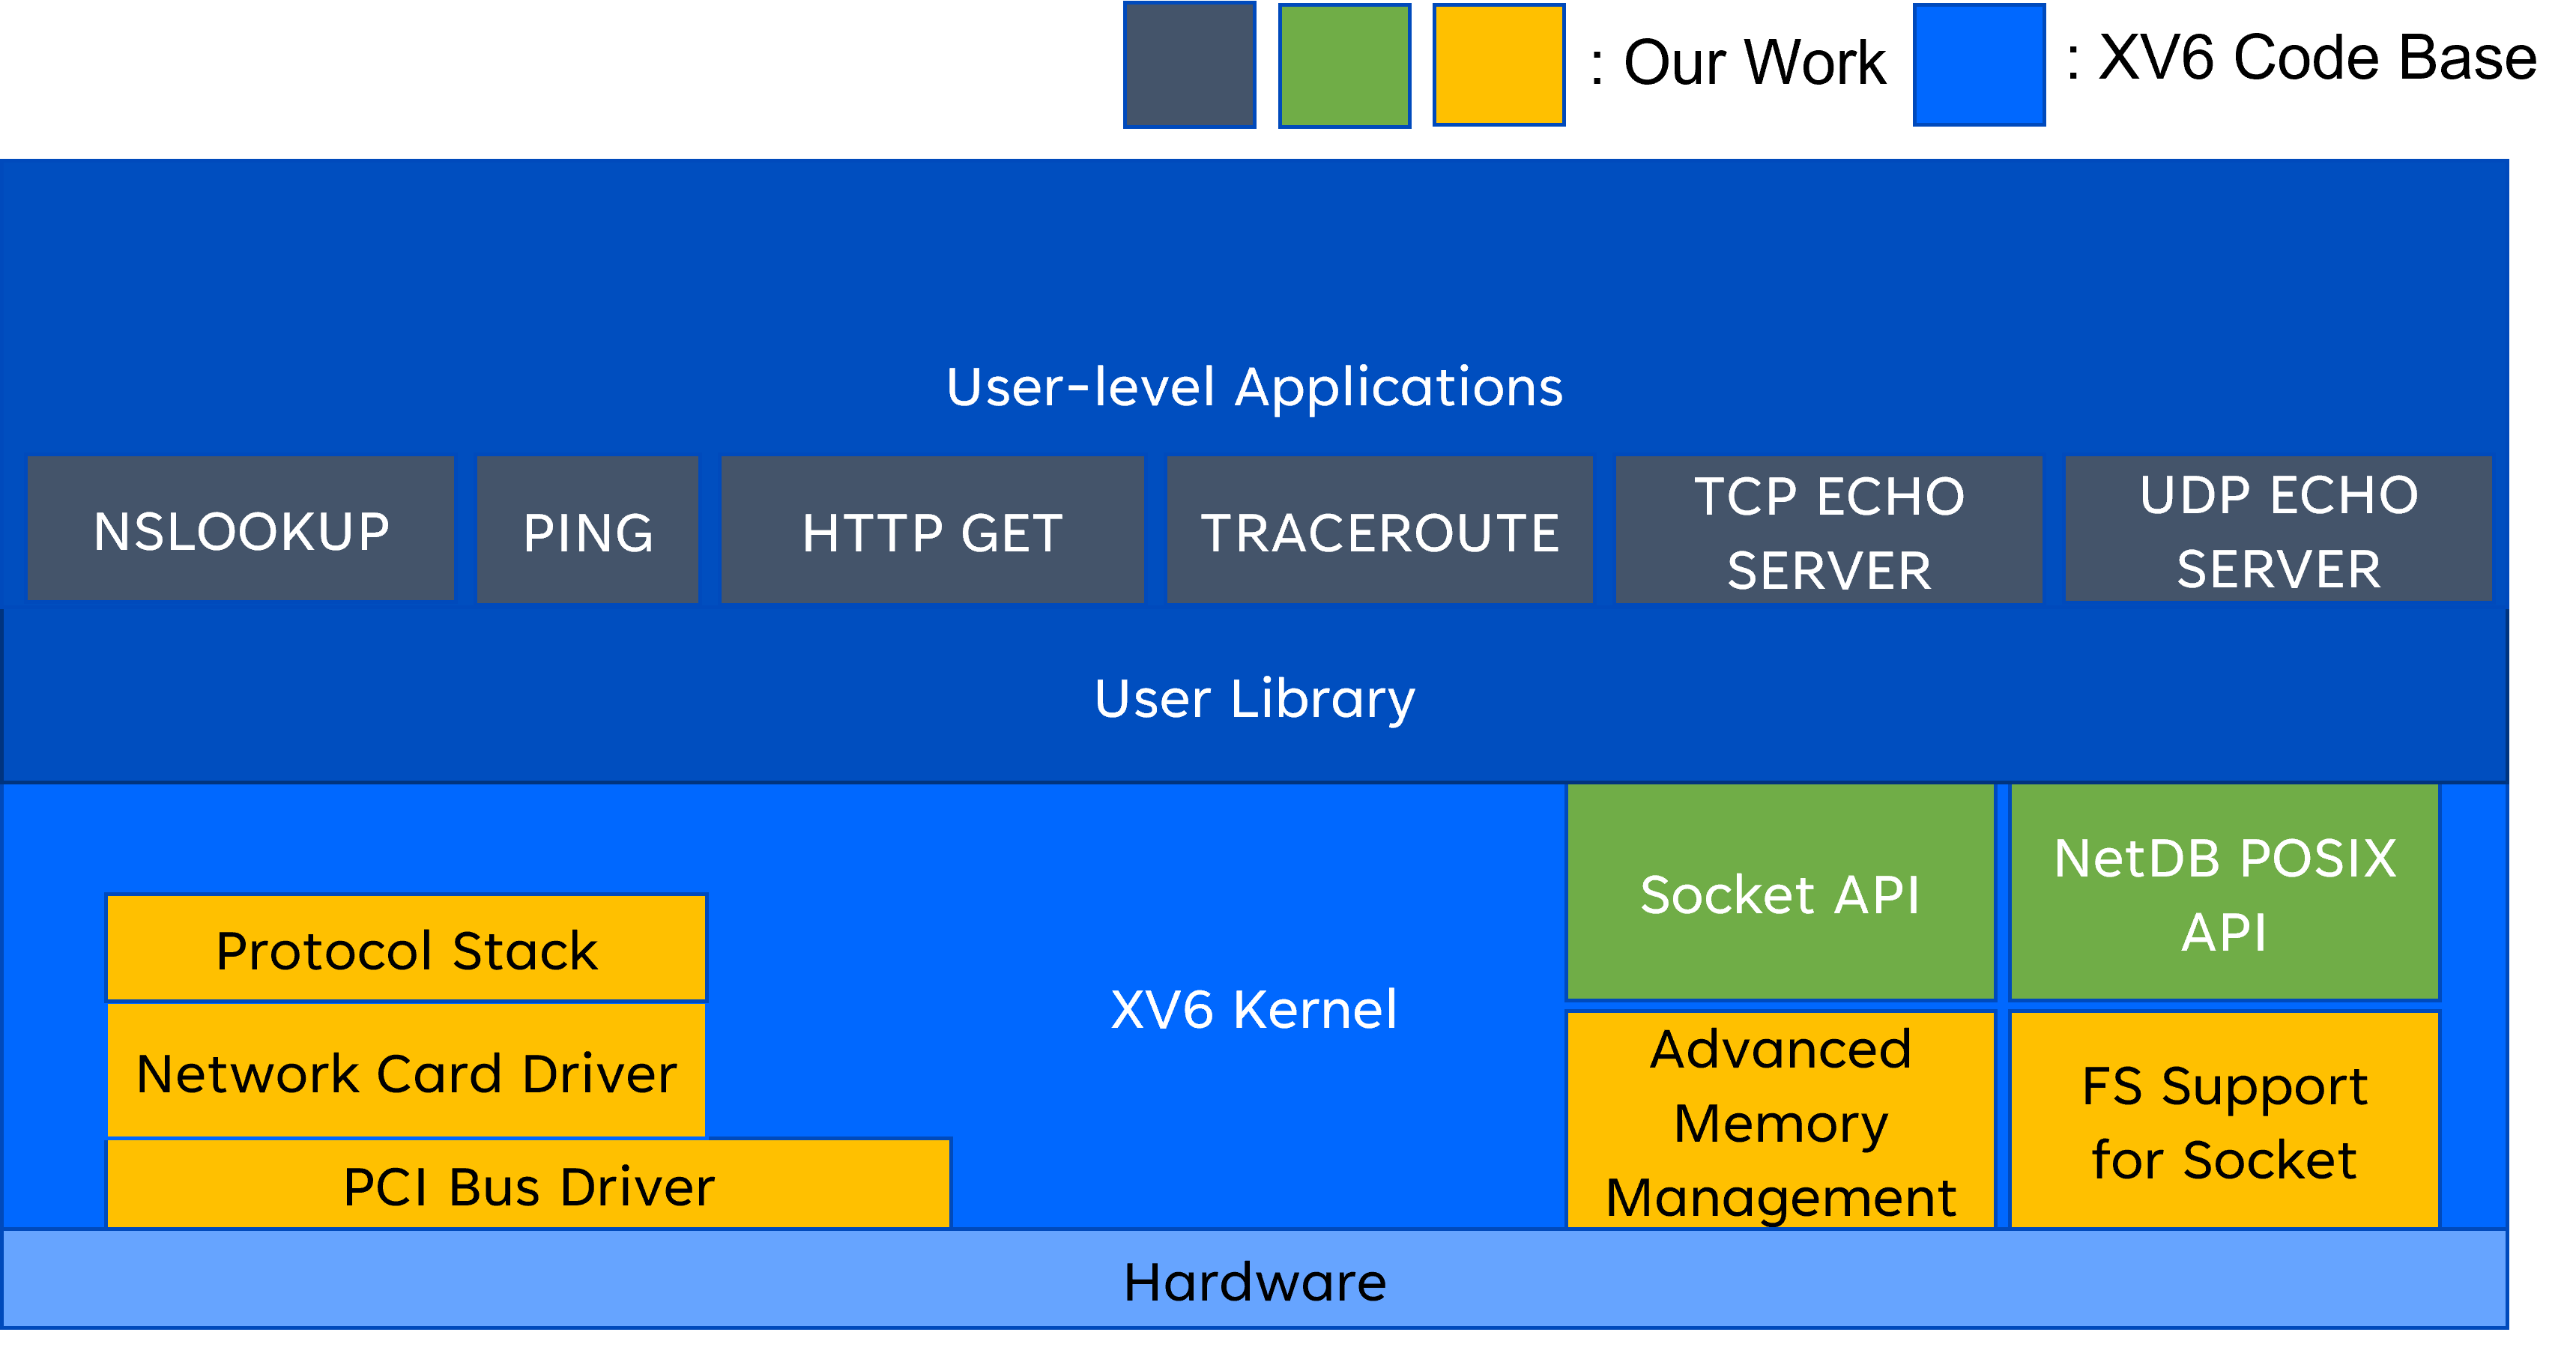
\includegraphics[width=0.8\textwidth]{arch.png}
	\caption{项目架构}
	\label{fig:arch}
\end{figure}

在内核态中的部分按功能分,可以分为三个部分:

一是负责处理实际数据收发、通讯的部分,自下而上分别是PCI总线的驱动、e1000网卡的驱动程序、基于LWIP的网络协议栈。
二是作为向上层提供服务的部分,包括提供一套数据收发原语的Socket API、提供一套使用DNS服务的接口的POSIX NetDB API部分。
三是围绕网络子系统内存分配频繁、动态内存分配要求高的需求、Socket API与类UNIX操作系统的文件系统部分结合紧密的特点,对内核进行的改进。
例如对内存分配的改进、对文件系统的改进、引入了与Linux内核中实现方式类似的链表等基础数据结构。

在内核和用户之间,用户态库也需要进行相应接口的实现。我们实现了Socket API和用于查询DNS的接口,例如
\texttt{gethostbyaddr}和\texttt{gethostbyname}的用户态库接口。
这些接口完全符合POSIX标准。

在用户态,我们实现了两类的应用程序:

第一类是用来调试、检验基础功能的应用程序。包括TCP、UDP的Echo Server、测试和远程主机实际通信以及DNS的
RFC 867日期时间服务客户端。
第二类是常用的网络实用程序,包括nslookup、ping、traceroute、httpget等。

\section{设备驱动程序的实现}

\subsection{PCI总线的驱动}

通用串行总线(PCI)是一种用于确保高性能、低开销的传输的本地总线。PCI总线的组件和卡片接口时处理器无关的,
因此该总线结构可以被多种处理器架构利用。

为了初始化PCI总线,需要驱动程序访问PCI配置空间,从而获取PCI设备的基本信息,例如设备的ID、设备的基地址等。
访问PCI配置空间有两种方式,但只有访问I/O端口的方式是符合标准的。这种方式使用两个32位的I/O端口,一个用于
指定配置地址,一个用于读写配置数据。配置地址的格式如图~\ref{fig:pci_config_addr}所示。
\begin{figure}[htb]
	\centering
	\caption{PCI配置地址的格式}
	\label{fig:pci_config_addr}
	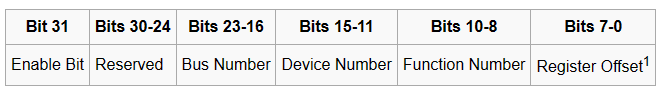
\includegraphics[width=0.5\textwidth]{controlreg.png}
\end{figure}
据此,我们实现的PCI驱动程序在代码\texttt{kernel/pci.c}中,它会访问PCI配置空间,获取PCI设备的基本信息,然后
加入设备表中。为了保证该驱动程序的可扩展性,我们的实现将不同驱动程序实现的相应初始化程序注册到数组中,如代码~\ref{code:pcireg}。
\begin{lstlisting}[numbers=left,style=CppStyle,caption={PCI驱动程序的初始化程序注册},label={code:pcireg}]
struct pci_driver pci_attach_vendor[] = {
	{0x8086, 0x100e, &e1000_nic_attach},
	{0x1af4, 0x1000, &virtio_nic_attach},
	{0, 0, NULL},
};
\end{lstlisting}
当驱动程序初始化的时候,每当注册新设备,都会在其中查找相应的初始化程序,然后调用该初始化程序。查找的方式
是读取设备类和设备ID,分别位于配置空间的偏移0x0b和0x0a中。如果找到相应的初始化程序,就调用该初始化程序。

当PCI驱动程序完成后,操作系统启动时,会调用\texttt{pci\_init}函数,该函数会遍历所有的PCI设备,完成
上述功能,并输出设备的基本信息。输出的信息如图~\ref{fig:initpci}所示。
\begin{figure}[htb]
	\centering
	\caption{PCI设备的基本信息}
	\label{fig:initpci}
	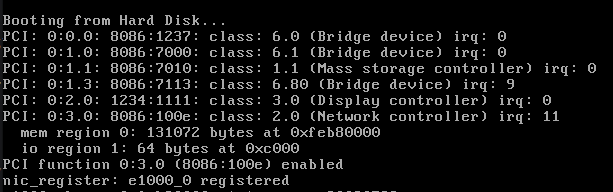
\includegraphics[width=0.5\textwidth]{initpci.png}
\end{figure}


\subsection{e1000网卡的驱动程序}

有了上述PCI驱动程序和相应扩展架构的实现。我们就可以实现e1000网卡的驱动程序了。e1000网卡的驱动程序的
重要组成部分是网卡的初始化程序,该程序会初始化网卡的寄存器,设置相应信息,使网卡进入可用状态。

\subsubsection{网卡的初始化}

有了完善的PCI驱动程序,e1000网卡的初始化在操作上就是对相应寄存器地址的读写。方法是调用PCI驱动程序
的\texttt{pciw}和\texttt{pcir}函数,分别用于写和读。初始化大致分为以下几个步骤:

\begin{enumerate}
	\item 从PCI配置空间中读取网卡的基地址寄存器,得到网卡的基地址。
	\item 从e1000的eeprom中读取MAC地址。
	\item 设置多播表为全0。
	\item 设置接受和发送的缓冲区等相关设置。
\end{enumerate}

由于本项目并没有要求大批数据的收发,只需要基本功能,因此e1000网卡工作在轮询模式下,不使用中断。
e1000网卡的收、发分别使用64、16个物理内存页作为缓冲区,其中每两个Receive Descriptor和Transmission Descriptor
共用一个缓冲区,因此每个缓冲区的大小是2KB。这样划分可以较好地保证缓冲区的对齐。

驱动程序完成后,会在启动时输出网卡相关的硬件信息,如图~\ref{fig:initnet}所示。
\begin{figure}[htb]
	\centering
	\caption{网卡的硬件信息}
	\label{fig:initnet}
	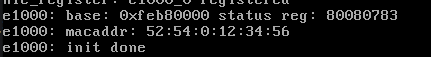
\includegraphics[width=0.5\textwidth]{inite1000.png}
\end{figure}
52:54:00:12:34:56是QEMU默认的虚拟网卡MAC地址,可见实现是正确的。

\subsubsection{网卡的收发}

从网卡收发数据是通过写相应的Read/Transmission Descriptor而实现的。默认情况下,这些Descriptor的Status
字段为0,表示准备好接收或发送数据。当网卡收到数据时,会将数据写入相应的缓冲区,并将Status字段置为0,
命令字段设置RS和EOP,表示数据已经正确写入,要求网卡回报状态。然后再在相应的寄存器中写入使用的Descriptor
的编号。

之后,驱动程序轮询网卡的状态寄存器,当网卡的状态寄存器中的RD和TD字段都为1时,表示数据已经正确接收或发送。
其中发送部分的代码如代码~\ref{code:send}所示。
\begin{lstlisting}[numbers=left,style=CppStyle,caption=数据发送,label={code:send}]
int e1000_net_send(void *state, const void *data, int len)
{
	netdev_t *card = (netdev_t *)state;
	e1000_t *e1000 = (e1000_t *)card->priv;
	uint32 tail = pcir(e1000, E1000_TDT);
	struct TD *next_desc = &e1000->tx_descs[tail];

	if (!(next_desc->status & E1000_TXD_STAT_DD) && (next_desc->cmd & E1000_TXD_CMD_RS))
	{
		return -1;
	}

	if (len > PKTSIZE)
	{
		len = PKTSIZE;
	}

	memmove(e1000->tbuf[tail]->buf, data, len);
	next_desc->length = len;
	next_desc->status = 0;
	next_desc->cmd = (E1000_TXD_CMD_RS | E1000_TXD_CMD_EOP);

	pciw(e1000, E1000_TDT, (tail + 1) % E1000_TXDESC_LEN);
	while (!(next_desc->status & 0x0f))
	{
		microdelay(1);
	}
	return len;
}
\end{lstlisting}


\section{基于LWIP的网络协议栈}

由于网络协议栈的实现工作量巨大、相当复杂。我们采用了常用的LWIP作为协议栈。
该协议栈实现了常见用的TCP/IP协议,如IP、TCP、UDP、ICMP、ARP、DHCP、DNS等。
一方面,该协议栈较为轻量级,一方面,配置该库只需要在一头文件中定义相应的宏。
因此我们选择了该实现。

\subsection{LWIP的配置}

LWIP的配置主要是在\texttt{lwipopts.h}中进行的。该文件中定义了各种宏,用于控制LWIP的功能。

由于协议栈运行在内核态。因此在LWIP库的视角下,LWIP的代码工作在没有操作系统的模式下,因此,我们配置文件中
主要的定义如代码~\ref{code:lwipopts}所示。
\begin{lstlisting}[numbers=left,style=CppStyle,caption=LWIP配置,label={code:lwipopts}]
#define NO_SYS 1

#define LWIP_NETCONN 0
#define LWIP_SOCKET 0

#define LWIP_ARP 1
#define LWIP_DHCP 1
#define LWIP_DNS 1
#define LWIP_ETHERNET 1
#define LWIP_ICMP 1
#define LWIP_RAW 1
\end{lstlisting}
首先,我们关闭了LWIP的socket和netconn接口,因为它们不能工作在无操作系统模式(NO\_SYS)下,因此,我们
需要禁用这些功能,仅保留基础的功能,然后用基础的API实现我们的Socket等接口。

我们启用了ARP、DHCP、DNS、Ethernet、ICMP和RAW协议。这些协议对于Socket API和POSIX NetDB API的实现
是不可或缺的。

\subsection{LWIP依赖函数的实现}

NO\_SYS下的LWIP只依赖极少数的函数,这些函数主要是用于时间管理、和随机数生成。这些函数实现在\texttt{kernel/lib/lwip/os/}中的文件中。
分别是sys\_now和lwip\_rand。由于LWIP仅利用时间戳进行时间差的计算,不用于任何时间戳的标注。因此可以直接反馈系统时钟中断中
记录的Ticks。而随机数的生成,我们采用了的是简单的线性同余法。这种方法能使用位运算快速实现,有利于内核态代码的高效工作。
随机数生成的代码如代码~\ref{code:lwip_rand}所示。
\begin{lstlisting}[numbers=left,style=CppStyle,caption=LWIP随机数生成,label={code:lwip_rand}]
unsigned long lwip_rand(void)
{
	uint32 time = sys_now();
	static unsigned int z1 = 12345, z2 = 12345, z3 = 12345, z4 = 12345;
	unsigned int b;
	b  = ((z1 << 6) ^ z1) >> 13;
	z1 = ((z1 & time) << 18) ^ b;
	b  = ((z2 << 2) ^ z2) >> 27;
	z2 = ((z2 & time) << 2) ^ b;
	b  = ((z3 << 13) ^ z3) >> 21;
	z3 = ((z3 & time) << 7) ^ b;
	b  = ((z4 << 3) ^ z4) >> 12;
	z4 = ((z4 & time) << 13) ^ b;
	return (z1 ^ z2 ^ z3 ^ z4);
}
\end{lstlisting}


\subsection{LWIP的初始化和工作循环}

LWIP的主要工作都在\texttt{kernel/net/net.c}中完成。首先,在NO\_SYS模式下,要使用LWIP,需要用\texttt{netif->input}
函数将数据传递到LWIP中。需要注意的是,LWIP不原生支持并发,而XV6支持对称多处理器。因此,为了防止LWIP内部的数据结构出现
不一致的情况,我们对任何使用LWIP的上下文都使用同一自旋锁保护。这意味着只有一个进程能同时访问网络功能。
这虽然一定程度上降低了效率,但是是不可或缺的。

其次,为了驱动LWIP不断收取、分发、处理数据,需要不断调用\texttt{sys\_check\_timeouts}函数。因此,在xv6的IRQ0中断,即
时钟中断中,我们调用该函数。这样,LWIP就能初步正常工作了。

为了实现正常的收发数据,我们需要做好网卡驱动程序和LWIP的对接。在初始化时,我们为每一个网卡都创建一个\texttt{netif}结构体。
然后在其中设置网卡的MAC地址、IP地址、子网掩码、网关地址、MTU等信息。最后,我们调用\texttt{netif\_add}函数将该网卡加入LWIP
的网络接口列表中。这样,LWIP就能够使用该网卡了。

但在收发数据前,首先,我们需要获取合适的IP地址,而非要求用户手动输入,这符合现代操作系统的实际。因此我们使用了DHCP协议。
首先,调用LWIP的\texttt{dhcp\_start}函数,然后若未获取IP地址,就反复试图从网卡中读入数据并交给LWIP处理。这样,LWIP
最终就能正确地设置网卡的IP地址了。这时,正在启动的操作系统内核会输出获取的IP地址等配置信息。
这部分代码如代码\ref{lst:netadd}所示。
\begin{lstlisting}[numbers=left,style=CppStyle,caption=网卡初始化,label={code:netadd}]
void
netadd(int n)
{
	struct netif *new = &netif[n];
	netdev_t *card = find_card_by_id(n);

	int i;
	char addr[IPADDR_STRLEN_MAX], netmask[IPADDR_STRLEN_MAX], gw[IPADDR_STRLEN_MAX];

	if (!netif_add_noaddr(new, (void *)card, linkinit, netif_input))
	{
		panic("netadd");
	}

	new->name[0] = 'e';
	new->name[1] = 'n';

	netif_set_link_up(new);
	netif_set_up(new);

	cprintf("net %d: mac ", n);
	for (i = 0; i < ETH_HWADDR_LEN; ++i)
	{
		if (i)
		{
			cprintf(":");
		}
		if (new->hwaddr[i] < 0x10)
		{
			cprintf("0");
		}
		cprintf("%x", new->hwaddr[i]);
	}
	cprintf("\n");

	if (!card->opts->open || card->opts->open(card))
	{
		panic("netadd: cannot open device\n");
	}

	dhcp_start(new);
	/* wait until DHCP succeeds */
	while (!dhcp_supplied_address(new))
	{
		linkinput(new);
		sys_check_timeouts();
	}

	ipaddr_ntoa_r(netif_ip_addr4(new), addr, sizeof(addr));
	ipaddr_ntoa_r(netif_ip_netmask4(new), netmask, sizeof(netmask));
	ipaddr_ntoa_r(netif_ip_gw4(new), gw, sizeof(gw));
	cprintf("net %d: addr %s netmask %s gw %s\n", n, addr, netmask, gw);

}
\end{lstlisting}

在实际运行中,QEMU虚拟机下的xv6输出如图\ref{fig:netadd}所示。使用QEMU参数保存相应的
数据包,如图\ref{fig:dhcppacks}所示。可见,一个正确的、典型的DHCP过程正常完成了。
首先,没有配置好IP地址的网卡发送了一个DHCP Discover数据包,源地址是0.0.0.0。
然后位于10.0.2.2的DHCP服务器以广播的方式返回了一个DHCP Offer数据包,这时,
网卡继续以0.0.0.0作为源地址发送了一个DHCP Request数据包,请求DHCP服务器分配
IP地址。最后,DHCP服务器返回了一个DHCP ACK数据包,这时,网卡就能正确地获取到
IP地址、子网掩码和网关地址等重要信息。在此例中,分别为
10.0.2.15、255.255.255.0和10.0.2.2。

\begin{figure}[htb]
	\centering
	\caption{DHCP初始化}
	\label{fig:http}
	\begin{subfigure}{0.4\textwidth}
		\centering
		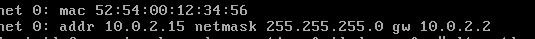
\includegraphics[width=\textwidth]{initproto.png}
		\caption{DHCP获取的内容}
		\label{fig:netadd}
	\end{subfigure}
	\begin{subfigure}{0.4\textwidth}
		\centering
		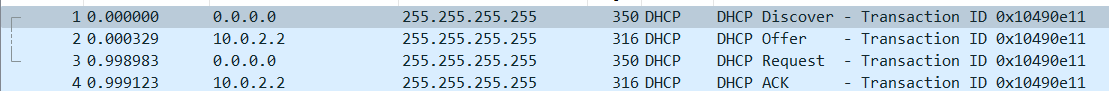
\includegraphics[width=\textwidth]{dhcppack.png}
		\caption{收发的数据包}
		\label{fig:dhcppacks}
	\end{subfigure}
\end{figure}

由于时钟中断不断驱动LWIP进行工作,当DHCP初始化完后,网卡立即发送、接受ARP数据包,
并且能够正常地进行网络通信。所捕捉的数据包如图\ref{fig:arppack}所示。
\begin{figure}[htb]
	\centering
	\caption{ARP数据包}
	\label{fig:arppack}
	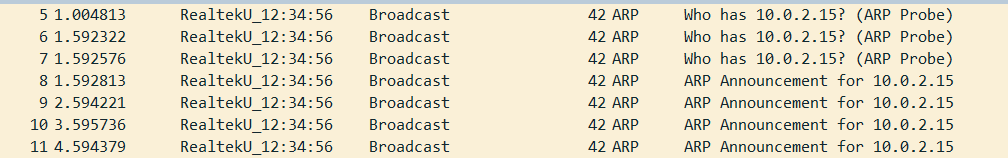
\includegraphics[width=0.8\textwidth]{arppack.png}
\end{figure}
此时,所有驱动程序和网络协议栈都可以正常地协同工作。为实现重要的用户编程接口
打下了良好的基础。

\section{Socket API}

Socket API是一组用于网络编程的接口,它是POSIX标准的一部分。它提供了一组函数,
来支持主要的用户程序间的通信功能,例如:
\begin{itemize}
	\item 设置和建立与其它网络中用户的连接;
	\item 向其它网络中用户发送数据、从其它网络中用户接收数据;
	\item 关闭连接、释放资源。
\end{itemize}
此外,它还能够提供一些高级的功能,例如:
\begin{itemize}
	\item 询问网络系统中的主机和状态;
	\item 按照其他用户的的要求,执行系统功能和控制功能;
\end{itemize}

在我们的项目中,Socket API处于核心位置,是耗费了最长时间、完成了最多代码的部分。

Internet Socket主要有三类:数据报套接字、流套接字和原始套接字。数据报套接字
提供了无连接的Socket服务,主要用于UDP协议;流套接字提供了面向连接的Socket服务,
常见的协议有TCP、SCTP等;原始套接字提供了对IP协议的完全访问,它允许用户构造任何
类型的IP数据包,包括IP头部和数据部分。前两种对典型的网络应用程序来说十分重要,
而原始套接字则是一种高级的功能,对我们在章节\ref{sec:netapp}中实现的网络应用程序nslookup、
ping和traceroute来说也相当重要,因此我们需要恰当第实现这三类套接字。

LWIP也提供了三种不同的API,分别为RAW IP API、RAW TCP API、RAW UDP API。它们提供了一层
较为“薄”的封装,提供了构造这三种类型数据包的基础接口。我们将借助它们实现Socket API。

注意到Socket类型和使用的协议不一定是一一对应的,例如,对于流套接字,
用户可以使用TCP协议也可以使用STCP。这样一来,我们并不应该在实现中将
利用不同协议的Socket实现耦合在一起,而应当进行逻辑上和实现上的分离,
这样才能保证这一部分的可扩展性和可维护性。

\subsection{架构设计}

首先,我们将Socket的基本操作定义在结构体\texttt{sockopt}中,如代码
\ref{lst:socketops}所示。
\begin{lstlisting}[numbers=left,style=CppStyle,caption=sockopts结构体,label={code:socketops}]
typedef struct sockopts
{
	struct
	{
		int type, protocol;
	} meta;

	int (*alloc)(struct socket *s);
	int (*connect)(struct socket *s, struct sockaddr *addr, int addrlen);
	int (*bind)(struct socket *s, struct sockaddr *addr, int addrlen);
	int (*listen)(struct socket *s, int backlog);
	int (*accept)(struct socket *s, struct socket *newsock, struct sockaddr *addr, int *addrlen);
	int (*send)(struct socket *s, void *buf, int len, int flags);
	int (*recv)(struct socket *s, void *buf, int len, int flags);
	int (*sendto)(struct socket *s, void *buf, int len, int flags, struct sockaddr *addr, int addrlen);
	int (*recvfrom)(struct socket *s, void *buf, int len, int flags, struct sockaddr *addr, int *addrlen);
	int (*close)(struct socket *s);

	int (*getsockopt)(struct socket *s, int level, int optname, void *optval, int *optlen);
	int (*setsockopt)(struct socket *s, int level, int optname, void *optval, int optlen);
} sockopts_t;
\end{lstlisting}
该结构体存储了一种针对特定“协议-Socket类型”二元组的Socket实现,它包含相应的元数据,以及一组函数指针。
它们将指向具体的Socket实现,例如,对于TCP流套接字,它们将指向TCP流套接字的实现。

每支持一种新的“协议-Socket类型”二元组,我们只需要实现相应的Socket实现,并将其注册到全局数组\texttt{sockopts}中,
它定义在文件\texttt{kernel/net/socket.c}中,如代码\ref{lst:sockopts}所示。
\begin{lstlisting}[numbers=left,style=CppStyle,caption=sockopts数组,label={code:sockopts}]
sockopts_t *sockopts[] = {
	&tcp_opts,
	&udp_opts,
	&raw_opts,
};
\end{lstlisting}
它显示了我们支持的三种“协议-Socket类型”二元组,分别是TCP流套接字、UDP数据报套接字和原始套接字。

每一个用户创建的Socket在内核中都会用一个\texttt{socket}结构体记录相应的参数,其中就有一个指针指向
\texttt{sockopts}数组中的某一项,这个指针在创建Socket时通过遍历上述数组来确定,如果无法找到,
就可以向用户汇报错误。\texttt{kernel/net/socket.c}中任何其他函数实现的主要部分都是根据该指针来调用相应的Socket实现。
并不实际处理通信的过程,而是将这些过程交给具体的Socket实现来处理,它们位于\texttt{kernel/net/tcpsock.c}、
\texttt{kernel/net/udpsock.c}、\texttt{kernel/net/rawsock.c}等具体的实现文件中。

这样,就完美实现了具有高度可扩展性的Socket实现。实现了不同协议、不同类型Socket实现在逻辑上和代码构成上的分离。
使得调试、维护、扩展都变得非常方便。

上述\texttt{sockopt}结构体中包含了几乎全部的Socket API的定义,但不是所有具体的Socket实现都能够实现全部的API。
对于那些不支持的操作,具体的实现只需要提供一个简单的、返回错误代码的函数实现即可。

下面,我们以UDP协议的数据报套接字为例,来介绍一种我们已经支持的协议和类型的Socket API的具体实现。

\subsection{Socket API实现(以UDP为例)}

UDP协议的套接字是数据报套接字,它的Socket实现定义在文件\texttt{kernel/net/udpsock.c}中。

首先,数据报Socket有一些操作不能执行,比如\texttt{listen}、\texttt{accept}、\texttt{connect}等操作,
根据上述分析,我们只需要在\texttt{udpsock.c}中提供一个简单的、返回错误代码的函数实现即可。
例如,\texttt{connect}操作的实现如代码~\ref{code:udpconnect}所示,它只是简单地返回一个错误代码。
\begin{lstlisting}[numbers=left,style=CppStyle,caption=UDP的\texttt{connect}实现,label={code:udpconnect}]
int udpconnect(struct socket *s, struct sockaddr *addr, int addrlen)
{
	return -EPROTONOSUPPORT;
}
\end{lstlisting}
按照POSIX标准,失败的操作返回-1,然后设置全局的\texttt{errno}变量。因此,我们在这里返回的是详细的错误代码,
而系统调用的实现函数会据此设置\texttt{errno}变量,然后返回-1。例如,\texttt{connect}系统调用的实现如代码~\ref{code:sysconnect}所示。
\begin{lstlisting}[numbers=left,style=CppStyle,caption=\texttt{connect}系统调用实现,label={code:sysconnect}]
int
sys_connect(void)
{
	struct file *f;
	int addrlen;
	struct sockaddr *addr;

	if (argfd(0, NULL, &f) < 0 || argint(2, &addrlen) < 0 || argptr(1, (void *)&addr, addrlen) < 0)
	{
		return -1;
	}
	if (f->type != FD_SOCKET)
	{
		seterror(-ENOTSOCK);
		return -1;
	}
	int err = socketconnect(f->socket, addr, addrlen);
	if (err < 0)
	{
		seterror(err);
		return -1;
	}
	return 0;
}
\end{lstlisting}

而对于那些可以执行的操作,我们需要提供一个具体的实现。这些实现会借助相应的LWIP协议栈的API来完成。
以UDP的\texttt{recvfrom}操作为例。为了实现该接口,有一些协议无关的操作和一些协议相关的操作。
协议无关的操作包括:
\begin{enumerate}
	\item 检查参数的合法性;
	\item 在调用之后、确实收到数据之前,将当前进程阻塞;
	\item 从LWIP的\texttt{pbuf}缓冲区中拷贝数据到用户空间;
\end{enumerate}
协议相关的操作包括:
\begin{enumerate}
	\item 为LWIP的UDP协议栈设置相关参数;
	\item 实现LWIP的接收回调函数;
\end{enumerate}
为了实现以上的操作,我们进行了如下的设计考量:
\begin{itemize}
	\item 由于网络操作等待时间较长,不应该进行循环式的“忙等”,因此应当将进程设为睡眠;
	\item 等待时间不能无限延长,同时Socket API也支持设置超时参数,因此应当处理超时;
	\item LWIP允许为所有事件设置一个处理函数,或者为特定的事件设置单独的回调函数。为了隔离不同的逻辑,我们选择后者;
\end{itemize}

协议相关的操作由UDP的Socket实现完成,代码如代码~\ref{code:udpsockrecvfrom}所示。
\begin{lstlisting}[numbers=left,style=CppStyle,caption=UDP Socket实现,label={code:udpsockrecvfrom}]
int udprecvfrom(struct socket *s, void *buf, int len, int flags, struct sockaddr *addr, int *addrlen)
{
	struct udp_pcb *pcb = (struct udp_pcb *)s->pcb;
	if (!pcb)
	{
		return -ECONNRESET;
	}

	netbegin_op();
	udp_recv(pcb, lwip_udp_recv_callback, s);
	netend_op();

	return 0;
}
\end{lstlisting}

而上述的协议无关的操作则由Socket API的顶层封装完成,代码如代码~\ref{code:sockrecvfrom}所示。
该段代码较长,我们将其放在\nameref{sec:appdixcode}中。

可见,该函数首先检查了参数,然后调用\texttt{skt->opts->recvfrom},对于一个UDP Socket,
该函数指针指向了UDP Socket的操作函数。该函数会调用\texttt{udp\_recv}注册回调函数,
并将Socket作为参数传递给回调函数。然后将当前进程置于休眠状态。

在回调函数中,会将接收到的数据包保存到Socket的接收缓冲区中,然后唤醒等待的进程。如
代码~\ref{code:lwipudprecv}所示。
\begin{lstlisting}[numbers=left,style=CppStyle,caption={LWIP的接受回调},label={code:lwipudprecv}]
static inline void lwip_udp_recv_callback(void *arg, struct udp_pcb *pcb, struct pbuf *p,
										  const ip_addr_t *addr, u16_t port)
{
	socket_t *socket = (socket_t *)arg;
	socket->recvfrom_params.recv_addr.sin_addr.addr = addr->addr;
	socket->recvfrom_params.recv_addr.sin_port = port;
	socket->recvfrom_params.recv_addr.sin_family = AF_INET;

	if (!p || p->tot_len > socket->recvfrom_params.recv_len)
	{
		if (p)
		{
			netbegin_op();
			pbuf_free(p);
			netend_op();
		}
		socket->recv_closed = TRUE;
		return;
	}
	// buffer hasn't been received
	if (socket->recv_buf)
	{
		return;
	}

	socket->recv_buf = p;
	socket->recv_offset = 0;

	socket->wakeup_retcode = 0;
	wakeup(&socket->recv_chan);
}
\end{lstlisting}


这样,可以灵活扩展的Socket \texttt{recvfrom}就实现了。其它的操作实现也类似。
其中,带休眠时间限制的休眠函数\texttt{sleepddl}可参见章节\ref{sec:kernel}
中的相关介绍。

其它协议Socket实现也是类似的,可参见源代码中的\texttt{kernel/net/tcpsock.c}、
\texttt{kernel/net/udpsock.c}、\texttt{kernel/net/rawsock.c}
等具体的实现文件,这里就不再赘述了。所有Socket API的测试都是与TCP/UDP Echo Server
配合完成的,可参见章节~\ref{sec:netapp}。

\section{POSIX NetDB API和DNS解析}

为了实现网络应用程序的方便,仅有Socket API是不够的。因为在现实场景中,用户极少会
指定IP进行操作,而是使用域名。因此,需要实现一个域名解析的功能,即DNS解析。

现代类UNIX系统中,经常使用的接口是\texttt{getaddrinfo}和\texttt{getnameinfo},
然而这组API的实现比较复杂,功能比较多,不利于我们形成可以正常运行的系统。因此,我们选择
实现较为传统的\texttt{gethostbyname}和
\texttt{gethostbyaddr}接口。这两个接口虽然已经
被POSIX标准弃用,但是实现简单、功能更为正交,因此更适合我们的实现。

\subsection{架构设计}

近年来,传统DNS解析的问题已经引发了广泛的关注。因此,新的DNS标准也正在普及,例如DNS over TLS、
DNS over HTTPS等。这些新的标准都是为了解决DNS的安全性问题,已经被Windows、Linux等主流操作系统
所支持。因此,考虑到未来的发展,我们的DNS实现的架构也应当具有可扩展性。

另一个需要考虑的问题是,\texttt{gethostbyname}和\texttt{gethostbyaddr}的返回值是连续的内存块,
其中变长内容由相对起始的偏移量表示,需要进行计算。因此,不把查询逻辑和构造返回值的逻辑分离开来,就会导致代码难以维护、
难以扩展。

因此,我们将DNS的基本操作抽象为一个\texttt{netdb\_proto}结构体,该结构体包含了DNS的基本操作,如代码~\ref{code:dnsop}所示。
\begin{lstlisting}[numbers=left,style=CppStyle,caption={DNS操作结构体},label={code:dnsop},language=C]
typedef struct netdb_proto
{
	void (*proto_init)();
	int (*proto_query)(char *name, netdb_query_type_t type, netdb_answer_t **answer);
	int (*proto_free_answer)(netdb_answer_t *answer);
	int (*proto_dump_answer)(const netdb_answer_t *answer);
	void (*proto_shutdown)();
} netdb_proto_t;
\end{lstlisting}
其中,\texttt{proto\_init}用于初始化DNS操作,\texttt{proto\_query}用于查询,\texttt{proto\_free\_answer}用于释放查询结果,
\texttt{proto\_dump\_answer}用于打印查询结果,\texttt{proto\_shutdown}用于操作系统内核关闭时的清理。

为了分离构造返回值的逻辑,我们底层的DNS实现将DNS的查询结果构造成一个\texttt{netdb\_answer}结构体组成的链表,该结构体包含了DNS的查询结果,
而系统调用的实现会进一步将该链表转换为合理的\texttt{hostent}返回值。

这样,架构设计就能实现高度的可扩展性,同时达到了模块中高内聚、模块间低耦合的目的。

\subsection{基本DNS查询的实现和测试}

普通DNS使用明文传输、基于UDP协议。我们利用LWIP的UDP RAW API实现了DNS数据的传输。

而构造DNS报文的过程则比较复杂,因为DNS将字符串部分进行了压缩,为了构造和解析DNS报文,
需要实现相应的解析逻辑。RFC 1035中对DNS报文的格式进行了详细的描述:
\begin{quote}
	In order to reduce the size of messages, the domain system utilizes a
compression scheme which eliminates the repetition of domain names in a
message.  In this scheme, an entire domain name or a list of labels at
the end of a domain name is replaced with a pointer to a prior occurance
of the same name.
\end{quote}
简而言之,DNS报文中的字符串部分会被压缩,压缩的方式是将字符串部分的每个子串都用一个指针指向之前出现过的子串,
高位的两位用于标识该指针是否指向字符串的开始,如果是,则该指针指向的是字符串的开始。代码~\ref{code:dnscompress}给出了字符串转化为正常字符串的实现。
\begin{lstlisting}[numbers=left,style=CppStyle,caption={字符串压缩解压缩},label={code:dnscompress},language=C]
static inline char *parse_dns_name(char *dst, char *name, char *ans)
{
	char *p = name;
	char *d = dst;
	char *s = ans;
	int len = 0;
	int i = 0;
	int offset = 0;
	int first = 1;

	while (*p != 0)
	{
		if ((*p & 0xc0) == 0xc0)
		{
			offset = (*p & 0x3f) << 8;
			p++;
			offset |= *p;
			p = s + offset;
			continue;
		}

		len = *p;
		p++;

		if (first)
		{
			first = 0;
		}
		else
		{
			*d = '.';
			d++;
		}

		for (i = 0; i < len; i++)
		{
			*d = *p;
			d++;
			p++;
		}
	}

	*d = 0;

	return p + 1;
}
\end{lstlisting}
然后,我们需要实现DNS报文的构造。该代码较长,因此我们将其放在了附录中,见\nameref{sec:appdixcode}
中的代码~\ref{code:dnsquery}。
接着,在LWIP UDP接收数据的回调函数中,我们实现了DNS回报的解析。这些部分大体就是对协议内容
的简单实现。

\texttt{proto\_query}的查询既要支持普通的DNS查询,也要支持从IP地址到域名的反向查询。但
该功能不需要实现额外的功能,RFC 1035中定义了一种特殊的域,即\texttt{in-addr.arpa},该域中的域名
用于IP到域名的反向查询。因此,我们只需要将IP地址转化为\texttt{in-addr.arpa}域中的域名,然后进行
正常的DNS查询,并取结果中的PTR记录即可。RFC中的相关描述如下:
\begin{quote}
	The Internet uses a special domain to support gateway location and
	Internet address to host mapping.  Other classes may employ a similar
	strategy in other domains.  The intent of this domain is to provide a
	guaranteed method to perform host address to host name mapping, and to
	facilitate queries to locate all gateways on a particular network in the
	Internet.
\end{quote}
由于本函数实现过长,故不在报告中完整呈现,请参见源代码中\texttt{kernel/net/baredns.c}
中的相关内容。

基本DNS功能的测试依赖于用户应用程序\texttt{nslookup}的实现,具体数据和内容见应用程序章节的~\nameref{sec:nslookup}小节。
该API连通此命令一同测试,能够正常工作。

\section{内核改进}
\label{sec:kernel}

\subsection{内存分配改进}

原始的xv6内核中,内存分配只有\texttt{kalloc}和\texttt{kfree}两个函数,分别用于分配和释放内核内存。该
函数的作用是按页分配内存,每次分配的内存大小为一页,即4KB。这种分配方式存在两个问题:
\begin{enumerate}
	\item 由于每次分配的内存大小为一页,因此分配的内存大小不可控,如果需要分配的内存大小不是一页的整数倍,那么就会造成内存浪费。
	\item 当分配超过一页时,难以保证分配的内存是连续的。
\end{enumerate}
然而,在网络驱动程序、网络协议栈、Socket API等部分,需要频繁地进行内存分配,而且分配的内存大小不固定、分配的大小常常远小于
4KB。为了避免耗尽内存,提高内存分配的效率。需要改进内存分配的方式。

常见的类UNIX操作系统,例如Linux有更加复杂的内存分配机制。例如Buddy/Slab分配器,可以分配任意大小的内存块。其中Buddy分配器
分配2幂次大小的内存块,而Slab分配任意指定大小的内存块。这种分配方式的优点是可以分配任意大小的内存块,然而完整的实现相当复杂,
不利于我们按期完成项目。因此,我们采用了一种简单的内存分配方式,即利用xv6现有的分配器分配页大小的内存。然后使用Slab分配器
分配任意大小的内存块。具体的实现在\texttt{kernel/slab.c}中。

Slab分配器的原理是将内存分为多个大小相同的内存块,每个内存块称为一个Slab。Slab分配器维护一个Slab链表,每个Slab中都有一个
空闲链表,用于记录空闲的内存块。当需要分配内存时,Slab分配器从空闲链表中取出一个内存块,当需要释放内存时,Slab分配器将内存块
插入空闲链表。当Slab中的内存块全部被分配时,Slab分配器从Slab链表中取出一个Slab,当Slab中的内存块全部被释放时,Slab分配器
将Slab插入Slab链表。它们操作的内存空间均由xv6的分配器分配。

我们的实现接口大致于Linux相应组件的接口相同。\texttt{kernel/slab.h}中定义了Slab的存储结构,如代码~\ref{code:slab}所示。
\begin{lstlisting}[numbers=left,style=CppStyle,caption={Slab的存储结构},label={code:slab},language=C]
typedef struct slab
{
	kmem_cache_t *cache;
	size_t in_use;
	size_t next_free;
	void *objects;
	kmem_bufctl *bufctl;

	spinlock_t lock;

	list_head_t link;
} slab_t;
\end{lstlisting}
而这些Slab由称之为Cache的结构管理。Cache的存储结构如代码~\ref{code:cache}所示,在\texttt{kernel/include/slab.h}中。
\begin{lstlisting}[numbers=left,style=CppStyle,caption={Cache的存储结构},label={code:cache},language=C]
typedef struct kmem_cache
{
	list_head_t full, partial, free;

	list_head_t link;

	size_t obj_size, obj_count;
	uint flags;
	spinlock_t lock;

	char name[KMEM_CACHE_NAME_MAXLEN];
} kmem_cache_t;
\end{lstlisting}
有了这些结构,我们就可以实现\texttt{kmem\_cache\_create}、\texttt{kmem\_cache\_alloc}、\texttt{kmem\_cache\_free}等接口。

在这些接口之上,我们也实现了\texttt{kmalloc},来方便不创建对应Cache,只指定大小的内存分配。
这些接口在驱动程序、Socket API和DNS相关的实现中发挥了关键的作用。


\subsection{文件系统改进}

xv6没有常见的VFS结构,但是其文件系统实现包含了对不同类型的文件节点的初步支持。
由于Socket API在分配、关闭Socket时需要创建相应类型的文件节点来返回File Descriptor,
因此我们在xv6的文件系统实现上做了一些扩展。

\texttt{kernel/fs.h}中定义了文件节点的存储结构,如代码~\ref{code:file}所示。
\begin{lstlisting}[numbers=left,style=CppStyle,caption={文件节点的存储结构},label={code:file},language=C]

typedef enum file_type
{
	FD_NONE = 1,
	FD_PIPE,
	FD_DEVICE,
	FD_SOCKET,
} file_type_t;

typedef struct file
{
	file_type_t type;
	int ref; // reference count
	char readable;
	char writable;

	union
	{
		struct pipe *pipe;
		struct inode *ip;
	};
	uint off;
}file_t;

\end{lstlisting}
我们在类型中加入了\texttt{FD\_SOCKET},并在\texttt{union}中加入了\texttt{socket}成员。
这样就存储了Socket的相关信息。

负责处理文件节点的函数包括\texttt{file\_alloc}、\texttt{file\_close}、\texttt{file\_dup}等。
我们在相应函数中加入了对Socket的处理,调用Socket相关的具体实现,这里举一例说明,如代码~\ref{code:fileclose}所示。
\begin{lstlisting}[numbers=left,style=CppStyle,caption={file\_alloc函数的修改},label={code:fileclose},language=C]
void
fileclose(struct file *f)
{
	struct file ff;

	acquire(&ftable.lock);
	if (f->ref < 1)
	{
		panic("fileclose");
	}
	if (--f->ref > 0)
	{
		release(&ftable.lock);
		return;
	}
	ff = *f;
	f->ref = 0;
	f->type = FD_NONE;
	release(&ftable.lock);

	if (ff.type == FD_PIPE)
	{
		pipeclose(ff.pipe, ff.writable);
	}
	else if (ff.type == FD_INODE)
	{
		begin_op();
		iput(ff.ip);
		end_op();
	}
	else if (ff.type == FD_SOCKET)
	{
		socketclose(ff.socket);
	}
}
\end{lstlisting}

在这段代码中,遇到Socket类型的文件节点时,调用了\texttt{socketclose}函数
实现Socket专属的关闭逻辑。

\subsection{进程管理改进}

本项目中对进程管理的改进主要包含对信号的支持和对可设置超时时间的进程休眠的支持。
对信号的支持主要是便于调试。并且实现复杂、代码较长。因此在报告中不做叙述。可参见源代码中的
\texttt{kernel/proc.c}。这里主要介绍对可设置超时时间的进程休眠的支持。
该函数的实现在\texttt{kernel/proc.c}中,如代码~\ref{code:sleepddl}所示。
\begin{lstlisting}[numbers=left,style=CppStyle,caption={\texttt{sleepddl}的实现},label={code:sleepddl},language=C]

uint sleepddl(void *chan, struct spinlock *lk, uint duration)
{
	if (duration == 0)
	{
		sleep(chan, lk);
		return 0xffffffff;
	}

	myproc()->sleep.deadline = duration * tickspersecond;
	sleep(chan, lk);
	int ret = myproc()->sleep.deadline;
	myproc()->sleep.deadline = 0;
	return ret;
}
\end{lstlisting}

它与xv6原有的\texttt{sleep}函数非常相似,唯一区别在于,它可以设置一个超时时间。
在唤醒之后,会将剩余的时间返回。如果没有超时,返回十六进制值\texttt{0xffffffff}。

为了对唤醒时间进行计数,在xv6的调度器实现中,每当下一个时间片到来时,会遍历所有进程,
如果某进程使用了带超时时间的休眠,就将其剩余时间减一。如果剩余时间为零,就设置该进程为
可运行的进程。在不久的将来,该进程就会被调度、继续执行。

该代码片段如代码~\ref{code:tick}所示。
\begin{lstlisting}[numbers=left,style=CppStyle,caption={定时唤醒的实现},label={code:tick},language=C]
	if (p->state == SLEEPING && p->sleep.deadline > 0)
	{
		p->sleep.deadline--;
		if (p->sleep.deadline == 0)
		{
			p->state = RUNNABLE;
		}
	}
\end{lstlisting} 

该功能对Socket API的实现非常有用。在Socket API中,我们常常需要为休眠设置一个超时时间,
来避免进程因为等待数据而无限期地休眠。


\subsection{常用数据结构实现}

设备驱动程序、DNS的查询过程中,我们需要一些能够动态地插入和删除元素的数据结构。
因此,我们实现了Linux类似的侵入式链表。

侵入式(Intrusive)链表是一种链表的实现方式,它将链表的节点单独定义为一个结构体,
并将链表节点的指针作为结构体的成员,这是链表中相应的指针都处于数据的内部,所以称之为侵入式链表。

这种链表实现的好处在于可以用同一套链表操作函数来操作不同的具体数据。当需要从链表节点获取数据时,
可以通过结构体中内存偏移的计算来获取数据的指针,从而实现链表节点和数据的互相获取。
这种计算的方法在Linux内核中被称为\texttt{container\_of}。代码~\ref{code:containerof}给出了这种计算的实现。

\begin{lstlisting}[numbers=left,style=CppStyle,caption={container\_of宏的实现},label={code:containerof},language=C]
// offset of a struct member
#define offsetof(type, member)  __builtin_offsetof (type, member)

// get struct pointer from member
#define container_of(ptr, type, member) ({                      \
        const typeof( ((type *)0)->member ) *__mptr = (ptr);    \
        (type *)( (char *)__mptr - offsetof(type,member) );})
\end{lstlisting}

而其余的链表操作函数实现定义在\texttt{include/list.h}中。包括插入、删除、遍历等操作。
这些操作函数的实现都是基于\texttt{list\_head}结构体的。

\section{用户态库}

用户态库是用户态和系统调用实现间的“胶水”。它对用户提供了POSIX兼容的编程接口。将相关参数
按照系统调用的约定存入内存,然后调用INT 0x80中断,将控制权交给内核。用户态库的实现在
\texttt{lib/ulib}目录下。

由于在32位环境下,传参数不会用到寄存器,因此已经正确地将参数存入内存中,只需要使用int指令
调用相应终端即可,这部分代码实现在\texttt{lib/ulib/usys.S}中。如代码~\ref{code:usys}所示。
\begin{lstlisting}[numbers=left,style=CppStyle,caption={usys.S中的系统调用实现},label={code:usys}]
#define SYSCALL(name) \
  .globl name; \
  name: \
    movl $SYS_ ## name, %eax; \
    int $T_SYSCALL; \
    ret
\end{lstlisting}
这定义了一个宏,用于定义系统调用的实现。宏中的\texttt{SYS\_name}是系统调用的编号,\texttt{T\_SYSCALL}是中断号。

这样就可以简单地用系统调用的名称迅速定义大量的系统调用库函数接口了。


\section{应用程序}
\label{sec:netapp}

\subsection{nslookup}
\label{sec:nslookup}

\subsubsection{程序介绍}

nslookup是一个用来查询因特网域名服务器的程序。程序允许使用者向域名服务器查询一个域名或
地址的信息,通常被用来诊断域名解析系统的基本结构信息,查询域名解析是否正常工作,在网络
故障时排查网络问题。

\subsubsection{功能分析}

一个完整的nslookup程序拥有两种使用模式:交互式与⾮交互式。
交互式的nslookup允许用户交互式查询多个主机/域名信息,并且具有多种交互命令用于处理复杂的
需求、提升用户体验。而⾮交互式的nslookup只允许用户一次性查询单个主机/域名信息。⾮交互式
的nslookup也⽀持通过命令⾏指定参数。
本项⽬的⽬标是实现一个简易的nslookup程序,因此此程序只实现了nslookup的核⼼功能:⾮交互
式地对域名或地址进⾏查询,并向用户显示查询结果。

\subsubsection{程序实现}

在本项目开始时,我尝试通过如下方法实现程序的查询功能:
\begin{enumerate}
	\item 通过socket编程与域名服务器通信
	\item 构造DNS QUERY报文,向域名服务器发起域名查询请求
	\item 解析DNS RESPONSE报文,解析由域名服务器返回的主机信息
\end{enumerate}

但是该方法⾯对的最大的障碍是,由于DNS复杂的压缩规则,通过编程解析DNS REPLY报文实现难
度较⾼。

因此我最后通过调用内核中已经实现的函数:gethostbyname与gethostbyaddr,获得主机信息。内
核中,netdb.h中实现了一组用来获取主机信息的函数,其中包括gethostbyname与
gethostbyaddr。这组函数会返回一个保存有主机信息的hostent结构体。
其定义如下代码~\ref{code:hostent}所示。

\begin{lstlisting}[numbers=left,style=CppStyle,caption={hostent结构体定义},label={code:hostent}]
	struct  hostent { 
             char    *h_name;        /* official name of host */ 
             char    **h_aliases;    /* alias list */ 
             int     h_addrtype;     /* host address type */ 
             int     h_length;       /* length of address */ 
             char    **h_addr_list;  /* list of addresses from name 
server */ 
     }; 
\end{lstlisting}
   
程序具体实现如下:
\begin{enumerate}
	\item 首先通过命令行接受用户输入参数,并对用户输入作初步的输入检查
	\item 对于用户的输入,使用inet\_pton判断输入类型,对地址和域名分别处理
	\item 对于输入的域名,通过调用gethostbyname获取描述该主机的hostent结构体
	\item 对于输入的地址,通过调用gethostbyaddr获取描述该主机的hostent结构体
	\item 对于获取的hostent结构体,使用用户友好的形式输出显示。
\end{enumerate}

具体的运行效果如图~\ref{fig:nslookup}所示。
\begin{figure}[htb]
	\centering
	\caption{nslookup运行效果}
	\label{fig:nslookup}
	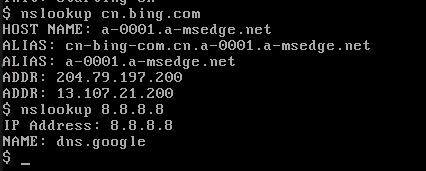
\includegraphics[width=0.8\textwidth]{nslookup.png}
\end{figure}
首先,对域名\texttt{cn.bing.com}进行查询,程序输出了该域名的所有IP地址,以及该域名的
的所有别名。然后,对IP地址\texttt{8.8.8.8}反向查询域名。该IP是谷歌的DNS服务器,程序
返回的域名为\texttt{dns.google}。可见,该程序是正确的。这其中产生的包如图~\ref{fig:nslookuppacket}所示。
\begin{figure}[htb]
	\centering
	\caption{nslookup产生的包}
	\label{fig:nslookuppacket}
	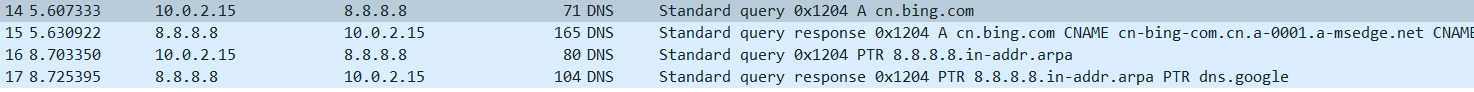
\includegraphics[width=0.8\textwidth]{nslookuppack.png}
\end{figure}
经过检查,以上程序的输出符合对应包的内容。尤其是DNS的回复,如图~\ref{fig:nslookuprep},
可以发现根据DNS规则进行了比较多的压缩,然而我们的程序依然正常地还原了域名。
\begin{figure}[htb]
	\centering
	\caption{nslookup过程的回复}
	\label{fig:nslookuprep}
	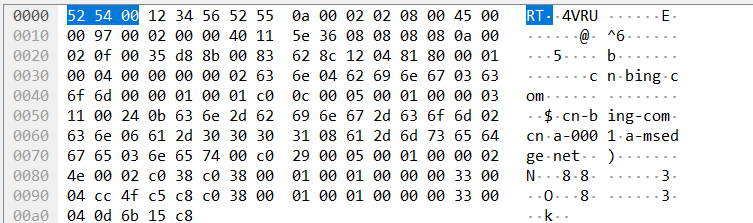
\includegraphics[width=0.4\textwidth]{nslookupresppack.png}
\end{figure}

\subsection{ping和traceroute}

\subsubsection{ping的实现}

利用原始套接字发送ICMP报文,将ICMP报文头的消息类型设置为8(ICMP request)。
ICMP\_HDR报文头如代码~\ref{code:ICMPHDR}所示。

\begin{lstlisting}[numbers=left,style=CppStyle,caption={ICMP\_HDR结构体定义},label={code:ICMPHDR}]
struct icmp_hdr {
	unsigned char type;		/* message type */
	unsigned char code;		/* type sub-code */
	unsigned short checksum;
	unsigned short id;
	unsigned short sequence;
	unsigned int timestamp;		/* not part of ICMP, but we need it */
};
\end{lstlisting}

然后,通过原始套接字实现的ICMP报文的发送,如代码~\ref{code:sendICMP}所示。

\begin{lstlisting}[numbers=left,style=CppStyle,caption={ICMP报文发送函数},label={code:sendICMP}]
struct sockaddr_in dest;
dest.sin_family = AF_INET;
dest.sin_port = htons(0);
dest.sin_addr.s_addr = ip;
char buff[sizeof(ICMP_HDR) + 32];
ICMP_HDR *pIcmp = (ICMP_HDR *) buff;
pIcmp->icmp_type = 8; 
pIcmp->icmp_code = 0;
pIcmp->icmp_id = (uint16_t) pID;
pIcmp->icmp_checksum = 0;
pIcmp->icmp_sequence = 0;
memset(&buff[sizeof(ICMP_HDR)], 'E', 32);
\end{lstlisting}

然后解析接收到的ICMP报文,判断是否为ICMP reply,如果是,则计算往返时间,否则丢弃并报错。
如代码~\ref{code:recvICMP}所示。
\begin{lstlisting}[numbers=left,style=CppStyle,caption={ICMP报文接收函数},label={code:recvICMP}]
ICMP_HDR *pRecvIcmp = (ICMP_HDR *) (recvBuf + 20); // (ICMP_HDR*)(recvBuf + sizeof(IPHeader));
IPHeader *ipHeader = (IPHeader *) recvBuf;
\end{lstlisting}
其中IPHeader结构体定义如代码~\ref{code:IPHeader}所示。
\begin{lstlisting}[numbers=left,style=CppStyle,caption={IPHeader结构体定义},label={code:IPHeader}]
	typedef struct IPHeader {
    uint8_t iphVerLen; 
    uint8_t ipTOS; 
    uint16_t ipLength; 
    uint16_t ipID; 
    uint16_t ipFlags; 
    uint8_t ipTTL; 
    uint8_t ipProtocol;
    uint16_t ipChecksum;
    uint32_t ipSource; 
    uint32_t ipDestination; 
} IPHeader;
\end{lstlisting}
由此可以显示相应的信息,如代码~\ref{code:ping}所示。
\begin{lstlisting}[numbers=left,style=CppStyle,caption={ping显示信息},label={code:ping}]
printf(" %d bytes from %s:", (int) nRet, inet_ntoa(from.sin_addr));
printf(" icmp_seq = %d. ", pRecvIcmp->icmp_sequence);
printf(" ttl = %d. ", ipHeader->ipTTL);
printf(" time: %d ms", (int) nTick - (int) pRecvIcmp->icmp_timestamp);
\end{lstlisting}

\subsubsection{traceroute的实现}

与ping类似,traceroute从1开始设置ttl,当报文每经过一个路由节点时,ttl减小1,当ttl为0时,节点丢弃报文,并向主机发送一个超时报文,报文的ip数据报中就有该节点的ip地址;随后增大ttl,获取下一个节点,就可以得知主机和目的地址之间的所有路由节点的ip地址

但是,因为部分节点不会响应icmp报文,发送超时报文,所以要为套接字设置超时。其中设置超时的代码如代码~\ref{code:settimeout}所示。
\begin{lstlisting}[numbers=left,style=CppStyle,caption={设置超时},label={code:settimeout}]
struct timeval timeout = {5,0};
setsockopt(sRaw,SOL_SOCKET,SO_RCVTIMEO,(char *)&timeout,sizeof(struct timeval));
\end{lstlisting}
而设置ttl的代码如代码~\ref{code:setttl}所示。
\begin{lstlisting}[numbers=left,style=CppStyle,caption={设置TTL},label={code:setttl}]
	setsockopt(sRaw, IPPROTO_IP, IP_TTL, &ttl, sizeof(ttl))
\end{lstlisting}

完成实现后,我们在xv6中运行ping,输出如图~\ref{fig:ping}所示。
\begin{figure}[htb]
	\centering
	\caption{ping输出}
	\label{fig:ping}
	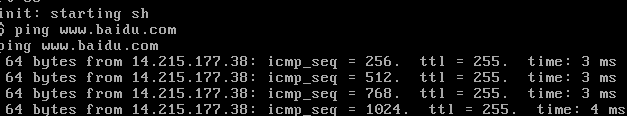
\includegraphics[width=0.6\textwidth]{ping.png}
\end{figure}
ping首先通过\texttt{gethostbyname}函数获取\texttt{www.baidu.com}的IP地址,
然后发送ICMP消息进行测试,并输出了四次结果。产生的报文如图~\ref{fig:pingpacket}所示。
\begin{figure}[htb]
	\centering
	\caption{ping产生的报文}
	\label{fig:pingpacket}
	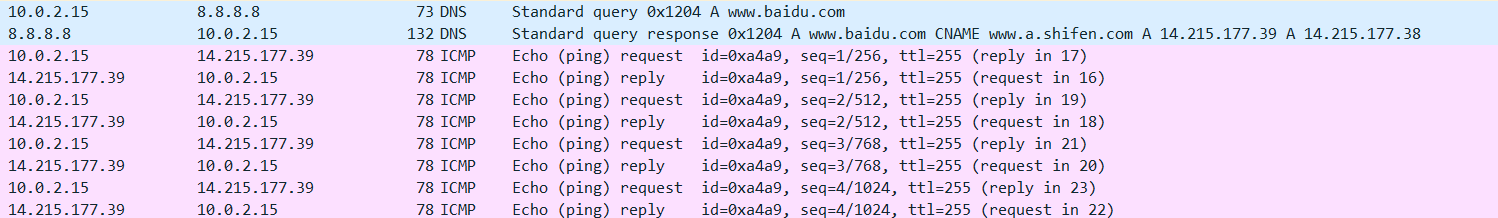
\includegraphics[width=0.6\textwidth]{pingpack.png}
\end{figure}
可见该过程是正常的。

\subsection{httpget}

httpget程序是wget的简化版,它向指定的服务器发送HTTP GET请求,获取服务器返回的数据,
然后将数据打印到标准输出。该程序的主要过程如下:
\begin{enumerate}
	\item 通过\texttt{gethostbyname}函数获取服务器的IP地址
	\item 通过\texttt{socket}函数创建套接字
	\item 通过\texttt{connect}函数连接服务器
	\item 通过\texttt{write}函数发送HTTP GET请求
	\item 通过\texttt{read}函数读取服务器返回的数据
	\item 将数据打印在标准输出流中。
\end{enumerate}
它的实现如代码~\ref{code:httpget}所示。
\begin{lstlisting}[numbers=left,style=CppStyle,caption={httpget实现},label={code:httpget}]
#include <user.h>
#include <netdb.h>
#include <socket.h>
#include <inet.h>

char host[64], buf[512];

int main(int argc, char **argv)
{
	const char *url, *path;
	ssize_t i, n;
	struct hostent *hp;
	int sockfd, r;
	struct sockaddr_in addr = {
		.sin_family = PF_INET, .sin_port = htons(80),
	};

	if (argc < 2)
	{
		printf(2, "usage: httpget url\n");
		return 0;
	}
	url = argv[1];

	path = strchr(url, '/');
	if (path)
	{
		memmove(host, url, path - url);
		host[path - url] = 0;
	}
	else
	{
		strcpy(host, url);
		path = "/";
	}

	printf(1, "host: %s, path: %s\n", host, path);
	hp = (struct hostent *)gethostbyname(host);
	//assert(hp, "gethostbyname");
	addr.sin_addr.s_addr = *(uint32_t *)hp->h_addr_list[0];
	printf(1, "* Trying %s (%s)\n", hp->h_name, inet_ntoa(*(struct in_addr *)&addr.sin_addr));

	sockfd = socket(PF_INET, SOCK_STREAM, IPPROTO_TCP);
	//assert(sockfd >= 0, "socket");

	r = connect(sockfd, (const struct sockaddr *)&addr, sizeof(struct sockaddr_in));
	//assert(r == 0, "connect");

	/* send http request */
	snprintf(buf, sizeof(buf), "GET %s HTTP/1.0\r\nHost: %s\r\nUser-Agent: curl\r\n\r\n", path, host);
	for (i = 0, n = strlen(buf); i < n;)
	{
		r = send(sockfd, buf + i, n - i);
		//assert(r > 0, "send");
		i += r;
	}
	write(1, buf, n);

	/* print http response */
	while (1)
	{
		n = recv(sockfd, buf, sizeof(buf));
		if (n <= 0)
		{
			break;
		}
		write(1, buf, n);
	}

	close(sockfd);
	return 0;
}
\end{lstlisting}

我们运行命令\texttt{httpget mba.xmu.edu.cn/favicon.ico},可以看到服务器返回的数据,如图~\ref{fig:favicon}所示。
由于请求的文件是二进制文件,因此打印出的内容不可读,但所返回的HTTP头部信息是可读的。可以发现我们的实现是正确的。
另外,使用命令\texttt{httpget www.kernel.org/doc/Documentation/x86/x86\_64/mm.txt},
可以看到服务器返回的数据,如图~\ref{fig:mmtxt}所示。由于该文件一般不可访问,因此服务器返回了一个HTML页面,
其中包含了301错误信息。可见,我们的实现能够正确完成HTTP请求。
\begin{figure}[htb]
	\centering
	\caption{httpget命令}
	\label{fig:httpget}
	\begin{subfigure}{0.4\textwidth}
		\centering
		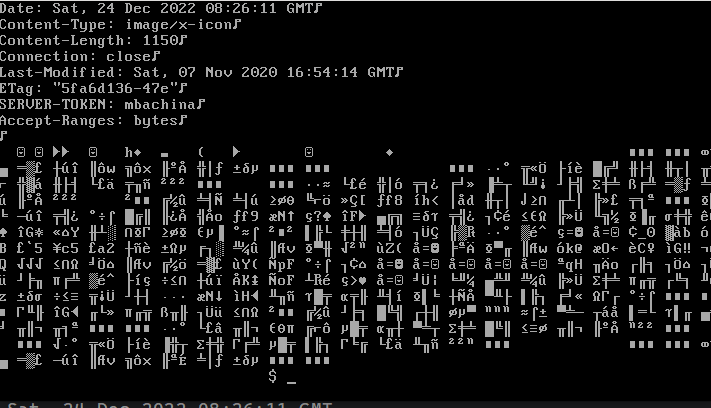
\includegraphics[width=\textwidth]{httpget1.png}
		\caption{favicon.ico}
		\label{fig:favicon}
	\end{subfigure}
	\begin{subfigure}{0.4\textwidth}
		\centering
		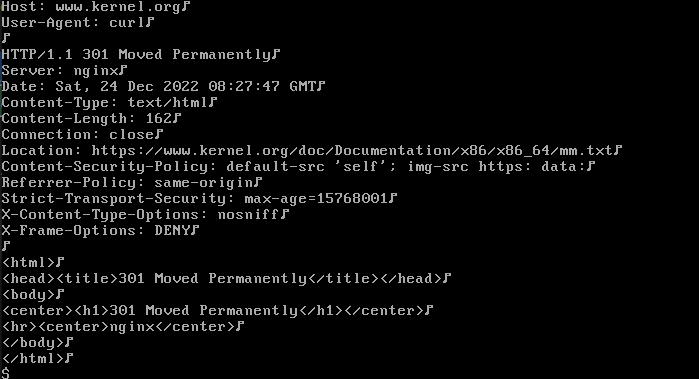
\includegraphics[width=\textwidth]{httpget2.png}
		\caption{mm.txt}
		\label{fig:mmtxt}
	\end{subfigure}
\end{figure}

其中通信过程中产生的数据如图~\ref{fig:httpgetpacket}所示。它符合典型的HTTP
1.0协议的通信过程,如图~\ref{fig:httpgetprocess};
经过仔细检查,协议头中的各个参数都进行了正确设置。如图~\ref{fig:httpgetheader}所示。
\begin{figure}[htb]
	\centering
	\caption{httpget命令产生的数据包}
	\label{fig:httpgetpacket}
	\begin{subfigure}{0.4\textwidth}
		\centering
		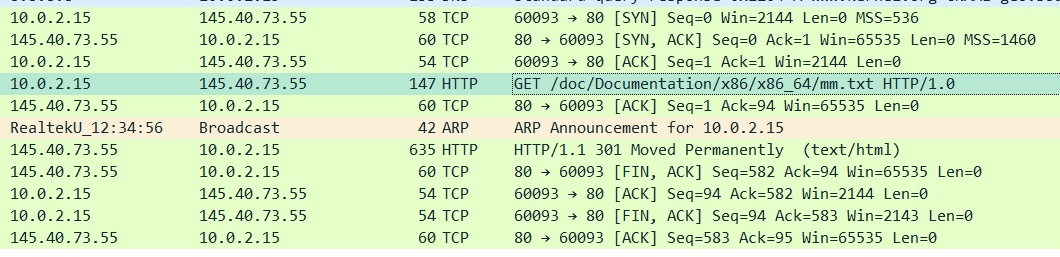
\includegraphics[width=\textwidth]{httpgetpack.png}
		\caption{通信过程}
		\label{fig:httpgetprocess}
	\end{subfigure}
	\begin{subfigure}{0.4\textwidth}
		\centering
		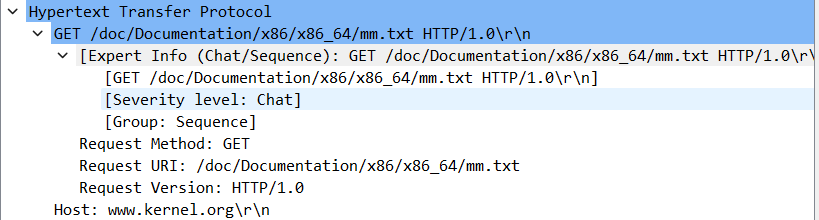
\includegraphics[width=\textwidth]{httpheader.png}
		\caption{发送的HTTP头部}
		\label{fig:httpgetheader}
	\end{subfigure}
\end{figure}

\subsection{RFC 867授时服务客户端daytime}

Daytime Protocol是1983年由RFC 867定义的,用于授时服务,客户端通过TCP连接或者到服务器,服务器
使用的端口号是13,服务器返回一个ASCII字符串,表示当前的时间,格式为:\texttt{Day Mon dd hh:mm:ss yyyy}

为了测试与远程服务器的连接,我们可以使用这个协议,客户端的代码如代码~\ref{code:datetime}所示。
该实现使用Socket编程,使用了TCP连接,连接到服务器后,发送一个空的数据包,服务器会返回一个32位的整数,表示从1900年1月1日到现在的秒数,
客户端可以通过这个时间戳来输出一个表示时间的用户可读的字符串。

\begin{lstlisting}[numbers=left,style=CppStyle,caption={daytime客户端},label={code:datetime}]
#define SERVER_PORT 13
#define SERVER_HOSTIP 0x2c8c8a80
char buf[512];

int main(int argc, char **argv)
{
//	struct hostent *hp;
	int sockfd, r;
	struct sockaddr_in addr = {
		.sin_family = PF_INET, .sin_port =  hton16(SERVER_PORT),
	};

	addr.sin_addr.s_addr = hton32(SERVER_HOSTIP);

	sockfd = socket(PF_INET, SOCK_STREAM, IPPROTO_TCP);

	r = connect(sockfd, (struct sockaddr *)&addr, sizeof(struct sockaddr_in));
	if (r < 0)
	{
		printf(1, "daytime: connect failed: %d\n", r);
		exit(-1);
	}

	ssize_t n;

	n = recv(sockfd, buf, sizeof(buf));
	if (n <= 0)
	{
		goto end;
	}

	write(1, buf, n); // stdout

end:
	close(sockfd);
	return 0;
}
\end{lstlisting}

该实现建立了一个TCP连接,连接到服务器后,发送一个空的数据包,服务器会返回一个
表示当前日期时间的ASCII字符串,客户端将其输出到标准输出。效果如图~\ref{fig:daytime}所示。
\begin{figure}[htb]
	\centering
	\caption{daytime客户端输出}
	\label{fig:daytime}
	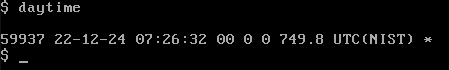
\includegraphics[width=0.6\textwidth]{daytime.png}
\end{figure}
位于\texttt{utcnist.colorado.edu}的日期时间服务器返回了调用时的日期时间。这其中产生的包
如图~\ref{fig:daytimepacket}所示。
\begin{figure}[htb]
	\centering
	\caption{daytime产生的报文}
	\label{fig:daytimepacket}
	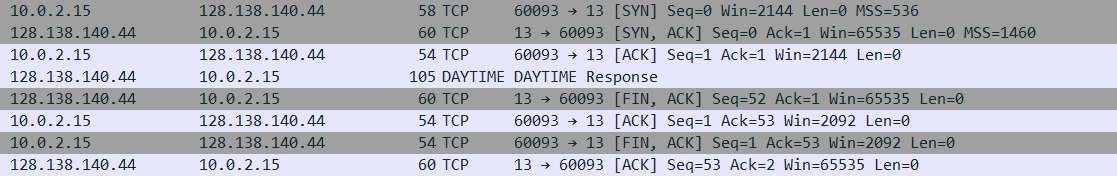
\includegraphics[width=0.6\textwidth]{daytimepack.png}
\end{figure}
可见这是一个典型的TCP连接、传输、断开的过程。我们的Socket实现正确处理了TCP连接的全过程。

\subsection{TCP和UDP的Echo Server}

在实现Socket API的过程中,我们需要简单易行的方式来测试我们的实现是否正确,
这里我们使用一个简单的Echo Server来测试我们的实现。

我们实现的TCP和UDP的Echo Server中使用TCP的代码如代码~\ref{code:echoserver}所示。
是一个单进程的简易Echo Server,在用于测试我们的Socket API的实现是否正确的用途
中发挥了重要的作用。

\begin{lstlisting}[numbers=left,style=CppStyle,caption={TCP Echo Server},label={code:echoserver}]
#include "types.h"
#include "user.h"
#include "socket.h"
#include "inet.h"

int
main(int argc, char *argv[])
{
	int soc, acc, peerlen, ret;
	struct sockaddr_in self, peer;
	unsigned char *addr;
	char buf[2048];

	printf(1, "Starting TCP Echo Server\n");
	soc = socket(PF_INET, SOCK_STREAM, IPPROTO_TCP);
	if (soc == 1)
	{
		printf(1, "socket: failure\n");
		exit(soc);
	}
	printf(1, "socket: success, soc=%d\n", soc);
	self.sin_family = AF_INET;
	self.sin_addr.s_addr = INADDR_ANY;
	self.sin_port = hton16(7);
	if (bind(soc, (struct sockaddr *)&self, sizeof(self)) == -1)
	{
		printf(1, "bind: failure\n");
		close(soc);
		exit(soc);
	}
	addr = (unsigned char *)&self.sin_addr;
	printf(1, "bind: success, self=%d.%d.%d.%d:%d\n", addr[3], addr[2], addr[1], addr[0], ntoh16(self.sin_port));
	listen(soc, 100);
	printf(1, "waiting for connection...\n");
	peerlen = sizeof(peer);
	acc = accept(soc, (struct sockaddr *)&peer, &peerlen);
	if (acc == -1)
	{
		printf(1, "accept: failure\n");
		close(soc);
		exit(soc);
	}
	addr = (unsigned char *)&peer.sin_addr;
	printf(1, "accept: success, peer=%d.%d.%d.%d:%d\n", addr[3], addr[2], addr[1], addr[0], ntoh16(peer.sin_port));
	while (1)
	{
		memset(buf, 0, sizeof(buf));
		ret = recv(acc, buf, sizeof(buf));
		if (ret <= 0)
		{
			printf(1, "EOF\n");
			break;
		}
		printf(1, "recv: %d bytes data received\n", ret);
		hexdump(buf, ret);

		if (send(acc, buf, ret) != ret)
		{
			printf(1, "send: failure\n");
			break;
		}
	}
	close(soc);
	return 0;
}
\end{lstlisting}

在QEMU中的xv6操作系统终端中执行\texttt{tcpecho}命令运行TCP Echo Server,结果如图~\ref{fig:tcpecho}所示。
\begin{figure}[htb]
	\centering
	\caption{TCP Echo Server}
	\label{fig:tcpecho}
	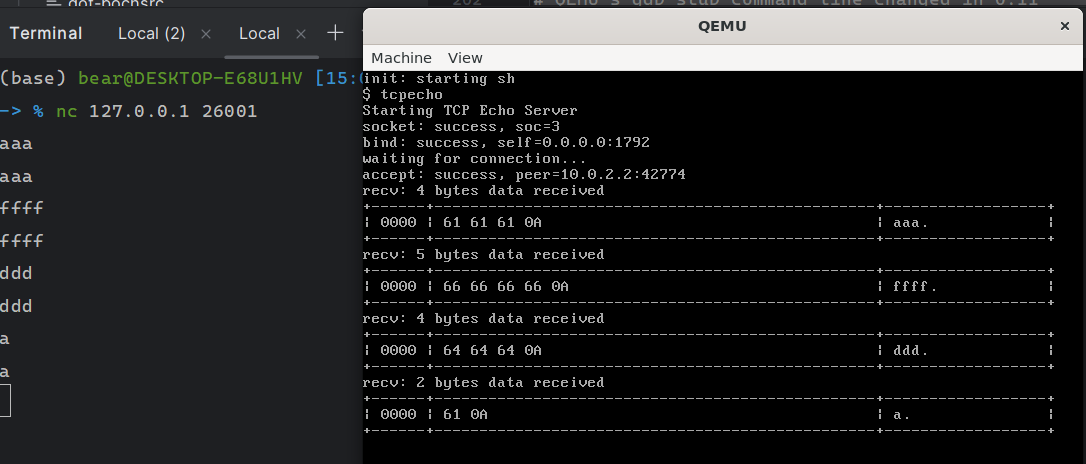
\includegraphics[width=0.8\textwidth]{tcpecho.png}
\end{figure}
可见,从宿主机终端中运行的\texttt{nc}命令向TCP Echo Server发送了的数据
都被TCP Echo Server将数据原样返回给客户端。同时TCP Echo Server也将收到的数据打印到了终端中。
包括数据包的基本信息。由捕捉的数据也可看出这一来往的过程。如图~\ref{fig:tcpechopack}所示。
\begin{figure}[htb]
	\centering
	\caption{TCP Echo Server和宿主机间往来的数据包}
	\label{fig:tcpechopack}
	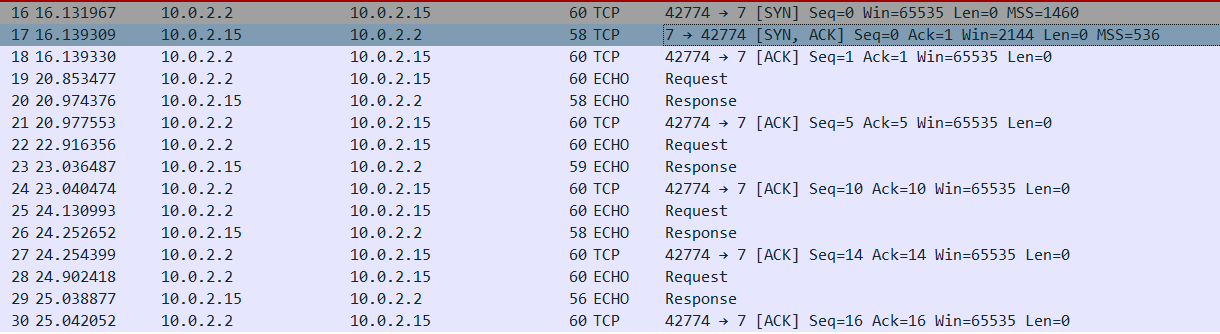
\includegraphics[width=0.8\textwidth]{tcpechopack.png}
\end{figure}



\chapter{项目管理}

\section{开发模式}

由于该项目规模较大、代码量高、开发周期短。因此,我们必须采用更有效的方式
管理项目的的源代码,进行源代码版本控制,防止某次更改导致大规模的错误。
此外,为了有效合并四个人合作的代码,我们也需要采用更有效的方式进行代码合并、
代码冲突的解决等。因此,我们采用了Git作为项目的源代码管理工具。

使用Git进行项目合作的流程如图~\ref{fig:gitflow}所示。
\begin{figure}[htb]
	\centering
	\caption{Git工作流程}
	\label{fig:gitflow}
	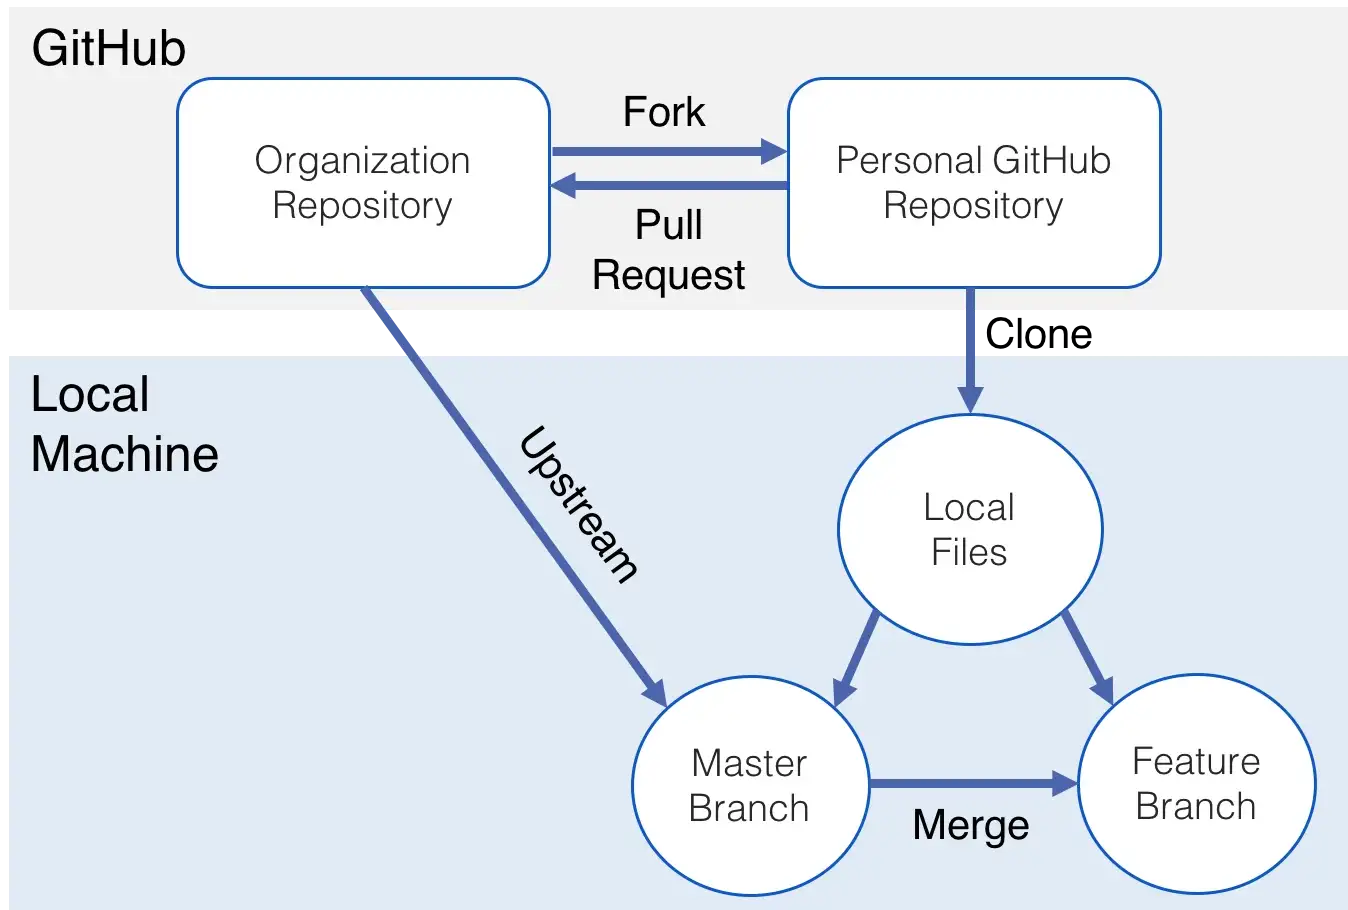
\includegraphics[width=0.8\textwidth]{git.png}
\end{figure}

\section{项目数据}
 

\chapter{项目感想}

\section{熊恪峥}

在这次计算机网络课程项目中,我负责了项目的设计、分工、全部内核态部分的实现和
少数用户态程序的实现。在这个过程中,我一方面增强了对xv6内核代码的理解,另一方面
也学习了现有成熟的网络API是怎么一步一步从0开始构建起来。从驱动程序如何将数据从
网卡中读出、从用户给定的位置送给网卡,到内核如何处理不同的网络协议,我自己编码
一步步将它们实现出来,这是一次非常有意义的经历。也让我对我们习以为常的“开箱即用”
的API接口的底层做什么、怎么做的问题有了更深的理解。

此外,由于我们项目中的代码量级极大,为了有效地管理,我们使用了git进行版本控制,
为了处理协议、Socket数据报类型等复杂的组合、灵活地复用代码,我不仅调查和研究了
现有操作系统内核相应的处理方式,也加入了自己在实践中积累经验得出的设计,这也让我
有很大的收获。

\section{赵淇奥}

在这次计算机网络课程设计项目中,我负责编写了nslookup程序。
这个程序的功能是向dns服务器查询给定的地址或域名。
在之前计网课程的实验中我多次接触过linux内置的该命令,而通过本次项目,亲自实现该命令,让我更加了解计算机网络编程、
熟悉计算机网络内核协议栈,并且对DNS的工作原理有了更深刻的认识。

\section{肖凯欣}

在项目中我负责编写ping程序和traceroute程序。在计算机网络的理论课上,这两个程序都作为网络层协议应用的示例。
在程序实现中需要我根据程序需要生成、发送相应的ICMP报文,并对收到的ICMP报文进行解析和处理。
在过程中我对于计算机网络编程,网络层协议以及ICMP协议的工作原理有了更加深刻的认识。

\section{谢哲涵}

在项目中我负责编写httpget程序。在计算机网络的实验课中,我们对使用HTTP连接获取互联网上的内容有了初步的理解和认识
,而在实现这个命令过程中我对于计算机网络编程,应用层协议有了更加深刻的认识。

\clearpage
\addcontentsline{toc}{part}{参考文献}

\bibliographystyle{unsrt}
\bibliography{reference}

\clearpage
\section*{附录:代码清单}
\addcontentsline{toc}{part}{附录:代码清单}
\label{sec:appdixcode}

\begin{lstlisting}[numbers=left,style=CppStyle,caption={DNS报文构造},label={code:dnsquery}]
static inline struct netdb_answer *make_query(char *name, int type)
{
	assert_holding(&netdb_lock);

	char *p = netdb_qbuf + 2048;

	dns_header_t *header = (dns_header_t *)p;
	header->xid = byteswap16(0x1204); // should be random though
	header->flags = byteswap16(0x0100); // Q, RD
	header->qdcount = byteswap16(1); // 1 question

	p += sizeof(dns_header_t);
	dns_question_t *question = (dns_question_t *)p;
	question->dnstype = byteswap16(type); // A or PTR
	question->dnsclass = byteswap16(1); // IN

	p += sizeof(dns_question_t);
	question->name = p;

	const uint8 hostlen = (uint8)strlen(name);
	memmove(question->name + 1, name, hostlen + 1);

	uint8 *prev = (uint8 *)question->name;
	uint8 count = 0;

	for (uint8 i = 0; i < hostlen; i++)
	{
		if (name[i] == '.')
		{
			*prev = count;
			prev = (uint8 *)(question->name + i + 1);
			count = 0;
		}
		else
		{
			count++;
		}
	}
	*prev = count;

	p = netdb_qbuf;
	size_t packet_len = sizeof(dns_header_t) + sizeof(dns_question_t) - sizeof(char *) + hostlen + 2;

	memmove(p, header, sizeof(dns_header_t));
	p += sizeof(dns_header_t);

	memmove(p, question->name, hostlen + 1);
	p += hostlen + 2;

	memmove(p, &question->dnstype, sizeof(question->dnstype));
	p += sizeof(question->dnstype);
	memmove(p, &question->dnsclass, sizeof(question->dnsclass));

	netbegin_op();
	struct pbuf *pbuf = pbuf_alloc(PBUF_TRANSPORT, packet_len, PBUF_RAM);
	if (!pbuf)
	{
		netend_op();
		return NULL;
	}
	memmove(pbuf->payload, netdb_qbuf, packet_len);
	query_ans = NULL;
	udp_recv(dns_pcb, netdb_dns_recv, NULL);
	err_t err = udp_send(dns_pcb, pbuf);

	if (err != ERR_OK)
	{
		netend_op();
		pbuf_free(pbuf);
		return NULL;
	}
	netend_op();

	if (!query_ans)
	{
		if (sleepddl(&dns_pcb, &netdb_lock, DNS_TIMEOUT) == 0)
		{
			return NULL;
		}
	}
	return query_ans;
}
\end{lstlisting}

\begin{lstlisting}[numbers=left,style=CppStyle,caption=Socket API的顶层封装,label={code:sockrecvfrom}]
int socketrecvfrom(socket_t *skt, char *buf, int len, int flags, struct sockaddr *addr, int *addrlen)
{
	if (skt->type == SOCK_STREAM)
	{
		if (addr)
		{
			return -EISCONN;
		}

		// as stated in the document, it will have the same effect as recv()
		return socketrecv(skt, buf, len, flags);
	}

	if (!skt->opts->recvfrom)
	{
		return -ESOCKTNOSUPPORT;
	}

	skt->recvfrom_params.recv_len = len;

	int err = skt->opts->recvfrom(skt, buf, len, flags, addr, addrlen);
	if (err)
	{
		return err;
	}

	if (skt->recv_buf == NULL)
	{
		acquire(&skt->lock);
		skt->wakeup_retcode = 0;
		if (sleepddl(&skt->recv_chan, &skt->lock, skt->recv_timeout) == 0)
		{
			release(&skt->lock);
			return -EWOULDBLOCK;
		}
		release(&skt->lock);

		if (skt->wakeup_retcode != 0)
		{
			return skt->wakeup_retcode;
		}
	}

	netbegin_op();

	len = pbuf_copy_partial(skt->recv_buf, buf, len, skt->recv_offset);
	skt->recv_offset += len;
	KDEBUG_ASSERT(skt->recv_offset <= skt->recv_buf->tot_len);

	if (skt->recv_offset == skt->recv_buf->tot_len)
	{
		pbuf_free(skt->recv_buf);
		skt->recv_buf = NULL;
		skt->recv_offset = 0;

		memmove(addr, &skt->recvfrom_params.recv_addr, sizeof(struct sockaddr_in));
		*addrlen = sizeof(struct sockaddr_in);
		addrin_byteswap((struct sockaddr_in *)addr);

		memset(&skt->recvfrom_params, 0, sizeof(skt->recvfrom_params));
	}

	netend_op();

	return len;
}
\end{lstlisting}


\end{spacing}

\end{document}